%%%%%% TODOs:
% put instructions on how to run my code (2 projects)
% put instructions on how to run the experiments?
%
%

\pdfoutput=1

\documentclass{l4proj}

%
% put any packages here
%
\usepackage{mathtools}
\usepackage{amsmath}
\usepackage{amssymb}
\usepackage{amsthm}
\usepackage{subcaption}
\usepackage{float}
\usepackage{array,multirow}
\usepackage{url}
\usepackage{hyperref}
\usepackage[table]{xcolor}
\usepackage{array}
\usepackage{booktabs}
\usepackage[toc,page]{appendix}
\usepackage[utf8]{inputenc}
\usepackage[acronym]{glossaries}


\usepackage{algorithm}
\usepackage{algpseudocode}
%\PassOptionsToPackage{noend}{algpseudocode}% comment out if want end's to show
\makeatletter
\def\BState{\State\hskip-\ALG@thistlm}
%\makeatother

% start with some helper code
% This is the vertical rule that is inserted
\newcommand*{\algrule}[1][\algorithmicindent]{\makebox[#1][l]{\hspace*{.5em}\vrule height .75\baselineskip depth .25\baselineskip}}%

\newcount\ALG@printindent@tempcnta
\def\ALG@printindent{%
    \ifnum \theALG@nested>0% is there anything to print
        \ifx\ALG@text\ALG@x@notext% is this an end group without any text?
            % do nothing
            \addvspace{-3pt}% FUDGE for cases where no text is shown, to make the rules line up
        \else
            \unskip
            % draw a rule for each indent level
            \ALG@printindent@tempcnta=1
            \loop
                \algrule[\csname ALG@ind@\the\ALG@printindent@tempcnta\endcsname]%
                \advance \ALG@printindent@tempcnta 1
            \ifnum \ALG@printindent@tempcnta<\numexpr\theALG@nested+1\relax% can't do <=, so add one to RHS and use < instead
            \repeat
        \fi
    \fi
    }%
\usepackage{etoolbox}
% the following line injects our new indent handling code in place of the default spacing
\patchcmd{\ALG@doentity}{\noindent\hskip\ALG@tlm}{\ALG@printindent}{}{\errmessage{failed to patch}}
\makeatother

\makeglossaries
\glstoctrue
\definecolor{Gray}{gray}{0.85}

\newcounter{example}[section]
\newenvironment{example}[1][]{\refstepcounter{example}\par\medskip
   \noindent \textit{Example~\theexample #1} \rmfamily}{\medskip}
\newtheorem{theorem}{Theorem}[section]
\newtheorem{lemma}[theorem]{Lemma}
\newtheorem{proposition}[theorem]{Proposition}
\newtheorem{corollary}[theorem]{Corollary}
\newtheorem{definition}{Definition}

\newcommand{\Lagr}{\mathcal{L}}
\newcommand{\fancyA}{\mathcal{A}}
\newcommand{\fancyI}{\mathcal{I}}
\newcommand{\fancyC}{\mathcal{C}}
\newcommand{\fancyP}{\mathcal{P}}
\newcommand{\fancyF}{\mathcal{F}}

\interfootnotelinepenalty=1000
%%%%%%%%% glossary entries and acronyms %%%%%%%%%%%%%%%%%%%%

%%% The glossary entry the acronym links to   
\newglossaryentry{apig}{name={API},
    description={An Application Programming Interface (API) is a particular set
of rules and specifications that a software program can follow to access and
make use of the services and resources provided by another particular software
program that implements that API}}
%%%%%%%%%%%
%%% define the acronym and use the see= option
\newglossaryentry{api}{name={API}, description={Application
Programming Interface}, first={Application
Programming Interface (API)\glsadd{apig}}, see=[Glossary:]{apig}}
%
\newglossaryentry{sip}{type=\acronymtype, name={SIP}, description={subgraph isomorphism problem}, first={Subgraph Isomorphism Problem (SIP)}}
%
\newglossaryentry{sat}{type=\acronymtype, name={SAT}, description={Satisfiable}, first={satisfiable (SAT)}}
%
\newglossaryentry{unsat}{type=\acronymtype, name={UNSAT}, description={Unsatisfiable}, first={unsatisfiable (UNSAT)}}
%
\newglossaryentry{graph}{type=\acronymtype, name={G}, description={graph}, first={graph (G)}}
%
\newglossaryentry{target}{type=\acronymtype, name={G$_{t}$}, description={target graph}, first={target (G$_{t}$)}}
%
\newglossaryentry{pattern}{type=\acronymtype, name={G$_{p}$}, description={pattern graph aka query}, first={pattern (G$_{p}$)}}
%
\newglossaryentry{patterns}{type=\acronymtype, name={P}, description={a set of pattern graphs aka queries}, first={pattern graphs (P)}}
%
\newglossaryentry{targets}{type=\acronymtype, name={T}, description={a set of target graphs aka database}, first={database (T)}}
%
\newglossaryentry{forwcheck}{type=\acronymtype, name={FC}, description={forward checking}, first={forward checking (FC)}}
%
\newglossaryentry{lds}{type=\acronymtype, name={lds}, description={label degree sequence}, first={label degree sequence ($lds$)}}
%
\newglossaryentry{nds}{type=\acronymtype, name={nds}, description={neighbourhood degree sequence}, first={neighbourhood degree sequence ($nds$)}}
%
\newglossaryentry{sn}{name={search node}, description={A search node denotes the number of recursive calls to the SIP algorithm taken to find a solution}}

\newglossaryentry{c}{name={candidate set ($\fancyC)$}, first={candidate set ($\fancyC$)}, description={todo}}

\newglossaryentry{tree}{name={tree}, description={A tree is an undirected graph such that any two vertices are connected by exactly one path. In this work, we refer to the vertices of the tree as \emph{nodes}.}}

\newglossaryentry{sufftree}{name={suffix tree}, description={A suffix tree S is a compressed trie containing all the suffixes of the given text as their keys and positions in the text as their values. It has the following properties: the tree has exactly n leaves numbered from 1 to n; except for the root, every internal node has at least two children; each edge is labeled with a non-empty substring of S; no two edges starting out of a node can have string-labels beginning with the same character; the string obtained by concatenating all the string-labels found on the path from the root to leaf i spells out suffix S[i..n], for i from 1 to n.}}

\newglossaryentry{canonicalform}{name={canonical form}, description={A canonical form of a graph G is a labeled graph Canon(G) that is isomorphic to G, such that every graph that is isomorphic to G has the same canonical form as G}}

\newglossaryentry{hashfunction}{name={hash function}, description={A function that can be used to map data of arbitrary size to data of fixed size. The values returned by a hash function are called hash values}}

\newglossaryentry{dfs}{name={depth-first search}, description={An algorithm for traversing or searching tree or graph data structures reported to be introduced by Charles Pierre Trémaux, a 19$^{th}$ century French mathematician. One starts at the root (selecting some arbitrary node as the root in the case of a graph) and explores as far as possible along each branch before backtracking}}

\newglossaryentry{hallset}{name={Hall set}, description={A set of \emph{n} whose domains include only \emph{n} values between them. Finding a Hall set allows for removing the values part of the hall set from the domains of variables that are not part of the Hall set.}}

\newglossaryentry{simd}{name={SIMD}, description={Single Instruction Multiple Data (SIMD) is a class of computers with multiple processing elements that perform the same operation on multiple data points simultaneously. Such machines exploit data level parallelism, but not concurrency: there are simultaneous (parallel) computations, but only a single process (instruction) at a given moment. }}

%%%%%%%%%%%%%%%% end of glossary and acronym entries %%%%%%%%%

\begin{document}
\title{Investigations of Subgraph Query Processing}
\author{Iva Stefanova Babukova}
\date{March 20, 2016}
\maketitle

\begin{abstract}


\end{abstract}

\educationalconsent
%
%NOTE: if you include the educationalconsent (above) and your project is graded an A then
%      it may be entered in the CS Hall of Fame
%
\tableofcontents
%==============================================================================
\chapter{Introduction}
\label{ch:introduction}
\pagenumbering{arabic}

This Chapter gives definitions and concepts used in this work and states the aims and motivations of the project. 

\section{Terminology, Definitions and Notations}
\label{sec:theory}
In this Section, we introduce all preliminary terminology and definitions used in this work. We start with basic introduction to graph theory, explaining the main problem that is discussed in this work, namely the subgraph isomorphism problem. Then, other concepts and notations are introduced, which are referred to later in this work.

\subsection{Graph Theory}
\label{sec:graphTheory}
%$Let \emph{V} be a finite set. Let \emph{E} be a subset of \emph{V} $\times$ \emph{V} and \emph{L} be a function, L: V $\rightarrow$ $\Lagr$, that assigns a label l $\in$ $\Lagr$ to each element in \emph{V}, where $\Lagr$ is the set of all possible labels. Then \emph{G} = (\emph{V}, \emph{E}, \emph{L}) is called a (undirected) graph if for any (\emph{v$_{1}$}, \emph{v$_{2}$}) $\in$ \emph{E} we have that (\emph{v$_{2}$}, \emph{v$_{1}$}) $\in$ \emph{E}.

A graph \emph{G} consists of a set of vertices V, a set of edges E, where each edge is a pair of vertices in V, and a \emph{labeling function} L: V $\rightarrow$ $\Lagr$ that assigns a label l $\in$ $\Lagr$ to each vertex in V, where $\Lagr$ is the set of all possible labels. Therefore, the set of all labels in \emph{G} is L(V(\emph{G})). We write V(\emph{G}) for the vertex set of \emph{G} and E(\emph{G}) for the set of edges in \emph{G}. By L(\emph{G}, \emph{v}) = x we mean that vertex \emph{v} in \emph{G} has label x.
We say that \emph{G} is \emph{undirected}, if every edge in E(\emph{G}) is an unordered pair of elements of V(\emph{G}). In this work, only undirected graphs are considered. The \emph{size} of \emph{G} is equal to the cardinality of E(\emph{G}), denoted as \emph{m}. The \emph{order} of \emph{G}, denoted as \emph{n}, is equal to the cardinality of V(\emph{G}).

\begin{example}
An example of undirected labeled graph is graph T on Figure \ref{fig:graphT}, where the labels of T are the colors of its vertices. L(V(\emph{T})) is equal to red (R), yellow (Y) and blue (B).
\end{example}

%% todo put these into an appropriate place
A \emph{sequence} is an ordered collection of objects in which repetitions are allowed. The \emph{length} of a sequence is equal to the number of its objects. The position \emph{i} of an element in a sequence  \emph{A} is called its index, denoted by \emph{A}[i]. 

\begin{example}
An example of a sequence of integers, ordered in non-decreasing order, is \{1, 2, 3, 4, 4\}.
\end{example}

A \emph{string} is a sequence of characters. Characters can be letters, numerical digits, punctuation marks, and whitespace.

Let \emph{A} and \emph{B} be sequences of integers. We say that \emph{B} is a \emph{subsequence} of \emph{A} if \emph{B} can be derived from \emph{A} by deleting zero or more elements in \emph{A}. A subsequence of a string is called a \emph{substring}.

\begin{example}
Let \emph{A} and \emph{B} be two sequences of integers, where \emph{A} = \{1, 2, 5, 3, 8\} and \emph{B} = \{2, 5, 3\}. Then \emph{B} is a subsequence of \emph{A}.
\end{example}

A \emph{path} in a graph is a sequence of distinct vertices, such that each successive pair of vertices are adjacent (i.e. connected by an edge). A \emph{cycle} is a path such that the first and the last vertices are adjacent. There may be zero, one or more distinct paths from vertex \emph{u} to vertex \emph{v} in \emph{G}. The \emph{length} of a path is equal to the number of its edges and the \emph{length} of a cycle is the number of its edges incremented by 1.

\begin{example}
An example of a path in graph T on Figure \ref{fig:graphT} is the sequence \{2, 3, 4, 5\}, which is a path of length 3. The path consisting of vertices \{2, 3, 8\} is an example of a cycle also of length 3.
\end{example}

The set of neighbours of a vertex \emph{v} in \emph{G} consists of all vertices adjacent to \emph{v}. The \emph{degree} of \emph{v} is the cardinality of its set of neighbours. By \emph{v} $\sim_{G}$ \textit{w} we mean that vertex \textit{w} is a neighbour of \emph{v} in \emph{G}. The set of neighbours of \emph{v} forms the \emph{neighbourhood} of \emph{v}, denoted as N(\emph{G}, \emph{v}). The neighbourhood degree sequence of \emph{v}, denoted nds(\emph{G}, \emph{v}), is a sequence consisting of the degrees of every neighbour of \emph{v}, taken in non-increasing order.

A graph \emph{G} is \emph{connected} if there exists a path between any pair of vertices in \emph{G}. An \emph{acyclic} graph has no cycles. A \emph{tree} is an acyclic connected graph. In this work, we refer to the vertices of the tree as \emph{nodes}.

\begin{example}
Graph T on Figure \ref{fig:graphT} is connected. Let use look at vertex 2. Its degree is equal to 3, because vertex 2 is adjacent to three vertices, namely 2 $\sim_{T}$ 1, 2 $\sim_{T}$ 3 and 2 $\sim_{T}$ 8. Consequently, N(\emph{T}, 2) = 1, 3, 8. nds(\emph{T}, 2) = \{8, 3, 1\}
\end{example}

\begin{figure}[H]
\centering
\begin{minipage}[t]{.3\textwidth}
  \centering
  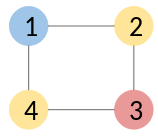
\includegraphics[height=2.1cm,width=2.3cm]{images/graphs/exampleGraph2.png}
  \caption{graph P}
  \label{fig:graphP}
\end{minipage}%
\begin{minipage}[t]{.4\textwidth}
  \centering
  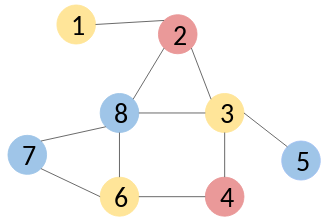
\includegraphics[height=3.4cm,width=5cm]{images/graphs/exampleGraph.png}
  \caption{graph T}
  \label{fig:graphT}
\end{minipage}%
\begin{minipage}[t]{.3\textwidth}
  \centering
  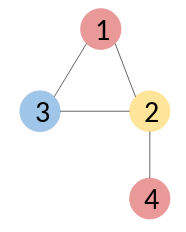
\includegraphics[height=3.4cm,width=3cm]{images/graphs/smalltarget.png}
  \caption{graph T1}
  \label{fig:graphT1}
\end{minipage}%
\caption{Instances of subgraph isomorphism problem (SIP)}
\label{fig:SIP}
\end{figure}

The \emph{density} of a graph \emph{G} measures what is the size of E(\emph{G}) compared to the maximum possible number of edges between the vertices in V(\emph{G}). Density for undirected graphs is calculated as follows:
\begin{equation}
\label{eq:graphdensity}
Density (\emph{G}) = \frac{2 \* m}{n(n - 1)}
\end{equation}

This formula is derived from the fact that the maximum number of edges that \emph{G} can contain is $\frac{n(|n - 1)}{2}$, when \emph{G} is a clique. If the \emph{m} is increased, while fixing the number of vertices as a constant, the density of \emph{G} becomes higher. Similarly, when \emph{n} is increased and \emph{m} is a constant, the density of \emph{G} becomes lower.

\begin{example}
The density of graph T, with 10 edges and 8 vertices, on Figure \ref{fig:graphT} is 2.3. % It is derived using formula \ref{eq:graphdensity}. %, $\frac{2.10}{8.7}$ is equal to 2.3.
\end{example}

\subsection{The Subgraph Isomorphism Problem}
A \emph{subgraph} of \emph{G} is a graph \emph{H} whose vertices and edges are subsets of the vertices and edges of \emph{G} and the labeling on the vertices is preserved.
%%% todo : change as adam says?
A \emph{non-induced subgraph isomorphism} is an injective mapping \emph{i} : \emph{P} $\rightarrow$ \emph{T} from a graph \emph{P} to a graph \emph{T} that preserves adjacency and labeling on vertices. That is, if \emph{v} $\sim_{P}$ \emph{w}, then \emph{i(v)} $\sim_{T}$ \emph{i(w)} and if L(\emph{P}, \emph{v}) = l, then L(\emph{T}, \emph{i(v)}) = l. The \emph{non-induced subgraph isomorphism problem} (SIP) is to find such a mapping from a given graph \emph{P}, called a pattern, to a given graph \emph{T} referred to as a target. The \emph{induced} SIP additionally requires that if \emph{v} $\nsim_{P}$ \emph{w} then \emph{i(v)} $\nsim_{T}$ \emph{i(w)}. In this work, we discuss only the non-induced version of SIP. We say that an instance of SIP is \emph{satisfiable} (SAT) if such a mapping \emph{i} exists and \emph{P} is said to be \emph{subgraph-isomorphic} to \emph{T}. Otherwise, the instance is \emph{unsatisfiable} (UNSAT).

\begin{example}
\label{ex:sip}
Consider graphs P and T in Figure \ref{fig:SIP}. The SIP instance between the pattern P (on the left-hand side of the Figure) and the target T (the graph on the middle of the Figure) is SAT- the mapping from P to T maps vertex 1 to vertex 8, vertex 2 to vertex 3, vertex 3 to vertex 4 and vertex 4 to vertex 6.
\end{example}

There are various existing algorithms for the subgraph isomorphism problem \cite{vf2,Solnon:2010,CP2015,Larrosa:2002,Bonnici:2013,Zampelli:2010,nauty}. More thorough analysis of the problem and discussion on existing work is presented in Section \ref{sec:sippatrick}.

\subsection{The Filtering-Verification Paradigm}
Let \emph{S} be the Cartesian product of a \emph{query set} \emph{Q} and a \emph{database} \emph{D}, where \emph{Q} contains patterns and \emph{D} contains targets. The process of solving the \gls{sip} for every pair in \emph{S} is referred to as the \emph{subgraph query processing} problem. The \emph{filtering-verification paradigm} is a subgraph query processing technique, executed for \emph{D} and \emph{Q}, that applies heavy \emph{filtering} procedures before the subgraph isomorphism algorithm execution in order to prune UNSAT instances.

\begin{example}
\label{ex:pathIndexing}
Consider Figure \ref{fig:SIP} and assume that graph P (in the left-hand side) is the query set, and graphs T (in the middle) and T1 (in the right-hand side) represent a database. Then, subgraph query processing would solve the SIP for instances (P, T) and (P, T1), where the former instance will be determined as SAT (Example \ref{ex:sip}) and the latter as UNSAT (there is no valid mapping from P to T1). 
\end{example}

\subsubsection{Filtering}

The first step of the filtering-verification paradigm is \emph{filtering}. During the filtering procedure, pruning algorithms are applied on the graphs in \emph{D} with respect to \emph{Q} in order to obtain the \emph{candidate set} \emph{C}. \emph{C} is a subset of \emph{D} and it contains all graphs that were not pruned by the applied filters. The second step, referred to as \emph{verification}, involves executing a \gls{sip} algorithm for every instance in the Cartesian product of \emph{Q} and \emph{C}.

In order to apply pruning algorithms on \emph{D}, a specific data structure has to be computed for both \emph{D} and \emph{Q}. This structure is known as \emph{index} and its definition is as follows: an \emph{index} of a set of graphs \emph{H}, denoted as $\fancyI_{H}$ is a collection of data, often stored in a file, that contains characteristics of the graphs in \emph{H}. The characteristics are called \emph{features}. Features can be represented in various ways. For instance, they could be paths, subtrees, cycles, or subgraphs. They are computed for every graph in \emph{H}. The first algorithm executed during the filtering stage is to compute such index for \emph{Q} denoted as $\fancyI_{Q}$ and \emph{D}, written as $\fancyI_{D}$\footnote{Unless it has already been computed.}. The process of computing the features of the graph to store them in the index is called \emph{feature extraction}.

The main reason why indices were introduced is \emph{reusability}. For instance, if $\fancyI_{D}$ has been computed during a previous execution of subgraph query processing with a different query set \emph{Q$^{\prime}$} and \emph{D} has not been changed, then one can reuse $\fancyI_{D}$. This would reduce the running time significantly\footnote{Results in Section \ref{subsec:ctindexEval} show that the bottleneck of the filtering-verification paradigm is the database index construction}. In theory, one could also reuse $\fancyI_{Q}$, but in practice this is rarely exploited. The set of queries \emph{Q} usually consists of much smaller number of graphs of lower order and smaller size than \emph{D}. This makes index computation much less expensive. Secondly, subgraph query processing with repeated query set rarely happens. 

There are many existing index computation and feature extraction techniques. Most common approaches are discussed later in this work. Example \ref{ex:index} illustrates an example approach.

\begin{example}
\label{ex:index}
Let \emph{D} be the database and \emph{Q} the query set defined in Example \ref{ex:pathIndexing} with the graphs on Figure \ref{fig:SIP}. Let the features be paths of length 2 represented as strings of concatenated vertex labels (yellow(Y), blue(B) or red(R)). The features of \emph{T}, \emph{T1} and \emph{P} are \{B-B, B-Y, R-Y, B-R\}, \{B-Y, R-Y, B-R\} and \{B-Y, R-Y\} respectively. The index of \emph{D}, $\fancyI_{D}$, is the union of the features of \emph{T} and \emph{T1} and the index of \emph{Q}, $\fancyI_{Q}$, consists of the features of \emph{P}. Note that the reverse of each of the strings is also a valid feature, as the graphs are undirected. Therefore, storing each feature and its reverse does not give additional structural information (in this case, this is equivalent to storing feature duplicates) for the cost of doubled index size. This is the reason why feature extraction algorithms enforce specific feature ordering requirements.
\end{example}

The procedure that follows after computing indices is referred to as \emph{candidates extraction}. A \emph{candidate set} $\fancyC$ of a database \emph{D} and a query set \emph{Q} is a subset of \emph{D} that contains all graphs that were not pruned by the applied filters. 
The purpose of filtering is to derive as small candidate set as possible in order to limit the of number calls to a subgraph isomorphism algorithm during verification. Note that the candidate set is a subset of \emph{D}. The worst case scenario is when $\fancyC$ and \emph{D} are equal, which means that filtering did not manage to prune any target graphs in \emph{D}.

\begin{example}
Taking the indices of \emph{D} and \emph{Q} computed in Example \ref{ex:index}, the candidate set $\fancyC$ consists of both T and T1 as each of them contains all features of \emph{P}.
\end{example}

\subsection{Verification}
Let \emph{S$^\prime$} be the Cartesian product of \emph{Q} and $\fancyC$, where $\fancyC$. \emph{Verification} is the process of solving the \gls{sip} for every pair of graphs in \emph{S$^\prime$}. All targets that do not contain the pattern, but were not rejected during the filtering step (i.e. they were included in the candidate set), are called \emph{false-positives}. The better the filtering technique, the lower number of false-positives it admits. The number of false-positives is often used as a measure of effectiveness of the filtering method \cite{foteini}.

The usage of the filter-verification paradigm is motivated by the fact that the decision version of the SIP is NP-complete \cite{Cook:1971}. Reducing the number of \gls{sip} calls by discarding targets that are \gls{unsat} for a given pattern without performing \gls{sip} call is believed to give opportunities for significant performance improvement \cite{ctindex,foteini}.
There are various subgraph query processing algorithms based on this paradigm \cite{ctindex,gcode,graphgrepsx,tree+delta>=graph,GRAPES}, which are discussed in more detail in Chapter \ref{ch:existingWork}. A thorough analysis of one of them is presented in Section \ref{sec:ctindex}.

\section{Aims of the project}
The subgraph query processing problem has a wide variety of applications in many fields, some of which include bioinformatics \cite{Bonnici:2013}, chemistry \cite{Regin:1995}, computer vision \cite{Damiand:2011,Solnon:2015}, law enforcement \cite{Coffman:2004}, model checking \cite{Calder:2015} and pattern recognition \cite{Conte:2004}. It involves repeatedly examining a large database, searching for graphs that contain particular patterns. For instance, in order to apply the best treatment for cancer, one might have to screen a patient's tumor to search for particular set of bio markers to identify the best course of treatment \cite{nature:2015}.

Filtering-verification paradigm is a new trend in Big Data research motivated by the fact that the decision version of the subgraph isomorphism problem is NP-Complete \cite{foteini,ctindex}. The subgraph isomorphism tests are reported as ``too time consuming'' \cite{foteini} and this is explained by the nature of the complexity of the subgraph isomorphism problem \cite{ctindex,foteini,freqStructBasedIndexing1}. Spending more time to build a database index and then reuse it for filtering with subsequent queries is shown in existing literature to ``... vastly improve search time and the up-front computation time is paid back quickly as repeated searches are performed'' \cite{fingerprints}.

In this work, we study subgraph query processing methods.  We first look at the approach to solving the problem employed by already existing work, i.e. the filtering-verification paradigm. We implement a framework that supports two different filtering techniques and carry out its empirical analysis. We then design a novel subgraph query processing approach based on the filtering-verification paradigm that does not employ an index structure, but uses fast simple filtering before a call to a SIP algorithm. Finally, the performance of the light filters approach is compared with the algorithms that use heavy index-bound filtering, and conclusions are made on the nature of the problem and the advantages of each method.

\section{Report organisation}
The remaining of this work is organised as follows. Chapter 2 presents review and analysis of existing approaches to solve the subgraph query processing problem, and the properties of 4 datasets used for testing and evaluation. The implementation and analysis of our framework consisting of two graph indexing and filtering methods is presented in Chapter 3. Chapter 4 describes a new approach to solve the subgraph query processing problem, which we call Light Filters. The evaluation of Light Filters and the analysis of the hardness of satisfiable and unsatisfiable subgraph isomorphism instances in the datasets are presented in Chapter 5. Chapter 6 provides a summary of this work and suggestions how to extend it in the future. 

%%%%%%%%%%%%%%%%%%%%%%%%% CHAPTER 2 %%%%%%%%%%%%%%%%%%%%%%%%%%%%
\chapter{Review of existing work}
\label{ch:existingWork}

\section{Datasets}
\label{sec:datasets}
This Section includes the specifications and the nature of the four datasets used for performance study of existing work in Section \ref{subsec:ctindexEval} and for evaluation in Section \ref{ch:evaluation}. The datasets are obtained from \cite{datasets}. Many related research publications use them to assess the performance of their subgraph query processing methods \cite{ctindex, gcode, graphgrepsx, tree+delta>=graph, GRAPES, lindex, foteini}. Therefore, running our experiments on these datasets makes our results easier to compare with existing work.

All four datasets consist of undirected labeled graphs. Each dataset has a set of target graphs, also called a database, and multiple sets of query graphs. Every graph has an id as well as every vertex in the graph. A description of each dataset is given below and the specifications of each dataset is shown in Table \ref{table:datasets}.

Aids is the standard database of the Antiviral Screen dataset of the National Cancer Institute. The database contains the topological structure of 40,000 chemical compounds, represented as graphs. The order of each graph is between 4 and 245. The graphs in this dataset are small and barely connected (Table \ref{table:datasets} shows that the average vertex degree is 2.1 and the average graph order is 45). This dataset has the largest number of unique labels, namely 62, and the largest database size.

Pcms contains 200 contact maps that represent relationships among amino acids. The graphs here are with much bigger order and higher density than the graphs in Aids, but they are still. Table \ref{table:datasets} shows that the graphs in Pcms have the highest density, which is 0.06, calculated using the Formula \ref{eq:graphdensity} defined in Chapter \ref{ch:introduction}. 

Pdbs consists of 600 target graphs, which represent proteins. The order of the graphs is 2,939 on average, where the graph with smallest order has 1,683 vertices and the graph with the biggest order has 7,979 vertices.

The fourth dataset is Ppigo and it has a database that consists of 20 protein interaction networks, where networks belong to species. This is the smallest dataset which also has the biggest graph order and size, which are both equal to 4,942 on average (Table \ref{table:datasets}).

Table \ref{table:dataSAT} shows the number and percent of \gls{sat} \gls{sip} instances for each dataset. For instance, Pdbs consists of large number of \gls{sat} problems (77.22\%), whereas Aids is the dataset with highest percent of \gls{unsat} problems (91.33\%).

\begin{table}
\centering
        \renewcommand{\arraystretch}{1.4}% Spread rows out...
        \begin{tabular}{l|r|r|r|r|}
\cline{2-5}
& \textbf{Aids} & \textbf{Pcms} & \textbf{Pdbs} & \textbf{Ppigo} \\
\cline{1-5}
\multicolumn{1}{|l|}{\# graphs}  & 40,000 & 200	& 600   & 20 \\
\hline
\multicolumn{1}{|l|}{\# disconnected graphs} & 3,157 & 200 & 360 & 20 \\
\hline
\multicolumn{1}{|l|}{\# unique labels} & 62 & 21 & 10 & 46 \\
\hline
\multicolumn{1}{|l|}{average graph order} & 45 & 377 & 2,939 & 4,942 \\
\hline
\multicolumn{1}{|l|}{average graph size} & 46.95 & 4,340 & 3,064 & 4,942 \\
\hline
\multicolumn{1}{|l|}{average density} & 0.05 & 0.06 & 0.01 & 0.01 \\
\hline
\multicolumn{1}{|l|}{average vertex degree} & 2.09 & 23.01 & 2.06 & 10.87 \\
\hline
\multicolumn{1}{|l|}{\# labels on average} & 4.4 & 18.9 & 6.4 & 28.5 \\
\hline
\end{tabular}
\caption{Characteristics of the datasets}
\label{table:datasets}
\end{table}

\begin{table}
\centering
        \renewcommand{\arraystretch}{1.5}% Spread rows out...
        \begin{tabular}{l|r|r|r|r|r|r|r|r|}
            \cline{2-9}
            &
             \multicolumn{2}{c}{\textbf{Aids}} & 
             \multicolumn{2}{|c}{\textbf{Pcms}} & 
             \multicolumn{2}{|c|}{\textbf{Pdbs}} & 
             \multicolumn{2}{c|}{\textbf{Ppigo}} \\
            \cline{2-9}
              & number  & percent & number & percent & number & percent & number & percent \\
              \hline
            \multicolumn{1}{|l|}{\textbf{all SIP calls}}  &240,000   &100 &1,800 &100 &3,600 &100 &100 &100 \\
            \multicolumn{1}{|l|}{\textbf{SAT SIP calls}}  &20,816 &8.67 &592 &32.8 &2,780 &77.22 &61 &61 \\
            \multicolumn{1}{|l|}{\textbf{UNSAT SIP calls}} &219,184 &91.33 &1,208 &67.2 &820 &22.78 &39 &39 \\
            \hline
        \end{tabular}
        \caption{The number of SAT/UNSAT SIP instances for each dataset}
        \label{table:dataSAT}
    \end{table}

\section{Filtering-Verification paradigm}
\label{sec:filterVerificationParadigm}
This Section gives an overview of already existing algorithms based on the filter-verification paradigm, defined in Section \ref{sec:theory}. Section \ref{subse:existingFVtechniques} discusses some of the existing filtering algorithms with respect to feature extraction and choice of features, Section \ref{subsec:verificationTechs} outlines the most commonly used subgraph isomorphism algorithms for verification.

\subsection{Existing Filtering Techniques}
\label{subse:existingFVtechniques}
There are two main types of feature extraction techniques, known as graph mining and exhaustive feature enumeration.

To explain what is meant by a graph mining technique, we introduce the following concepts. The \emph{support ratio} of a feature \emph{f} in a database \emph{D} is equal to the number of graphs in \emph{D} that contain \emph{f} divided by the total number of graphs in \emph{D}. A feature is \emph{frequent} if its support ratio is higher or equal to a certain algorithm-specific threshold value. \emph{Graph mining} techniques store only features which are considered as frequent in the database. Common graph-mining techniques include gIndex  \cite{freqStructBasedIndexing1}, fgIndex \cite{fg-index}, closure-tree \cite{closure-tree}, cpIndex \cite{cp-index}, L-Index \cite{lindex}, tree+$\Delta$ \cite{tree+delta>=graph} and TreePi \cite{treepi}.

\emph{Exhaustive feature enumeration} techniques store in the index all features of every graph in the database, regardless of their support ratio.
%Consequently, indices produced by such techniques are much larger than indices obtained through graph-mining algorithms and it takes more time to perform filtering, since there are more features to be iterated through. Exhaustive feature enumeration indices however are faster to compute since they do not have to calculate support ratios and feature frequency metrics.
Some well-known exhaustive feature enumeration techniques include \cite{graphgrepsx,ctindex,anotherindex,gcode}

Choosing a feature extraction method often depends on the type of datasets one has to work with. For instance, graph mining techniques are inefficient when the data in the database is frequently being changed \cite{freqStructBasedIndexing1}. When frequently inserting and deleting graphs in the database, the support ratio of the features may change and make the index outdated. Consequently, the index becomes less reusable and thus the total execution time of subgraph query processing is highly increased. Graph-mining techniques also take longer to built the database index since they spend additional time on calculating the support ratio of each feature. An advantage of graph mining techniques is that they require much less storage space than exhaustive feature enumeration algorithms, as only frequent features are stored in the index. This lowers the storage space requirements and makes the process of constructing the candidate set faster, since there are less features to be iterated through. 

There are various structures that can be used as features. Some of them include paths \cite{graphgrepsx,GRAPES}, trees \cite{closure-tree,treepi,ctindex}, subgraphs \cite{fg-index,anotherindex,cp-index,lindex,tree+delta>=graph} of the targets, or all of the aforementioned combined \cite{ctindex,tree+delta>=graph}. The choice of features influences the filtering performance. It is often a trade off in terms of time and filtering strength \cite{foteini}. This is further investigated in Section \ref{subsec:ctindexEval}, where we report on performance results obtained from an indexing method that uses a combination of paths, trees and graph cycles as features.

\subsection{Verification techniques}
\label{subsec:verificationTechs}
Most of the subgraph query processing methods that adopt the filtering-verification paradigm are mainly focused on improving the filtering stage, while reusing the same algorithm for verification, which is commonly VF2 \cite{vf2} \cite{foteini,ctindex,graphgrepsx,tree+delta>=graph}.
%%%%%%%%%%%%%%%%%%%%%%%%%%%%%%%%%%%%%%%%%%%%%%%%%%%%%%%%%%%%%%%%%%%%%%%%%%
%%                               CT-Index                               
%%%%%%%%%%%%%%%%%%%%%%%%%%%%%%%%%%%%%%%%%%%%%%%%%%%%%%%%%%%%%%%%%%%%%%%%%%
\section{CT-Index}
\label{sec:ctindex}

CT-Index \cite{ctindex} is an existing subgraph query processing approach that adopts the filter-verification paradigm. This method supports undirected graphs with edge and vertex labels and also wild card patterns. Although not explicitly stated in \cite{ctindex}, CT-Index addresses the non-induced subgraph isomorphism problem defined in Section \ref{sec:theory}. In this Section, we introduce and discuss the filtering algorithm and analyze its complexity in Section \ref{subsec:ctindexF}. Section \ref{subsec:ctindexV} explains the verification algorithm. Also presented is a complexity analysis of the algorithms used by CT-Index and an empirical study of its performance (using an open-source Java implementation) in Section \ref{subsec:ctindexEval}.

\subsection{Filtering}
\label{subsec:ctindexF}
During the filtering step, the features of all graphs in a database \emph{D} are extracted and saved to a file, i.e. the target index $\fancyI_{D}$. Features are specific subgraphs used to classify graphs, and are stored as hash-key fingerprints. Features may be paths, subtrees and/or cycles of bounded length. Since vertices may contain labels, these features can be viewed as strings from a specified alphabet (where the alphabet is the labels). In \cite{ctindex} it is stated that the reason for using \glspl{tree} and cycles (as well as paths) is that ``trees capture additional structural information" and cycles ``represent the distinct characteristic of graphs, often neglected when using only trees as features".

Although the time complexity of computing all features of a graph is not reported, it can be derived as follows. To extract a subtree of a graph \emph{G} with \emph{m} number of edges, one starts with initially empty tree and repeatedly adds edges to extend the vertices that are in the current tree via the recursive function \emph{ExtendTree}. We write \emph{F} for the set of every edge \emph{e} in \emph{G}, such that one of the vertices of \emph{e} is connected to is part of the current tree and the other is not. If we have \emph{n} number of vertices in the current tree, each with degree \emph{d}, then the size of \emph{F} is at most \emph{n(d - 1)}. \emph{ExtendTree} adds an edge specified as parameter to the current tree, generates \emph{F} and makes a recursive call for every edge in \emph{F}, until the tree reaches size \emph{m}.

In the start of the \gls{tree} extraction when adding the first edge to the empty tree, the vertices on both ends of the edge are also added as part of the tree. Therefore, the size of \emph{F} is \emph{2(d-1)} initially. After every recursive call, one more vertex is added to the tree, which introduces \emph{(d-1)} new edges. That makes a total of \emph{m + 1} vertices that will be added to the tree and \emph{(m + 1)(d - 1)} visited edges. Consequently, the complexity of extracting tree features is $\mathcal{O}(|E|(m + 1)(d - 1))$, where $|\emph{E}|$ is equal to the average size of a graph in \emph{D}. From this formula one can see that the the size of the graphs in \emph{D} has significant impact on the performance of the algorithm. When the graph density is high, the algorithm will be slower because of the high degree of each vertex.

CT-Index computes a unique representation of each distinct feature, its \emph{\gls{canonicalform}}, and stores its string encoding in $\fancyI_{D}$. Thus, the equality of two features can be checked by testing the equality of their canonical forms. The canonical label of a \gls{tree} feature is computed as follows: (1) find the root node \emph{r} of the tree, (2) impose a unique ordering of the children of each node. Step (1) is computed by repeatedly removing all leaf nodes of a \gls{tree} until a single node or two adjacent nodes remain. In the first case, \emph{r} is the last node left. In the second case the edge connecting the two remaining nodes are removed to obtain two \glspl{tree}, each with one of the remaining nodes as a root.
Step (2) is based on the ordering of edge and node labels. For each node \textit{p} that is a parent of nodes \textit{u} and \textit{v}, deciding whether \textit{u} is before \textit{v} depends first on the labels of the edges (p, u) and (p, v), then on the labels of \textit{u} and \textit{v} and finally on the subtrees of \textit{u} and \textit{v}. A bottom-up approach is used (i.e. start with the nodes in the lowest level and move up towards the root) to compute this.

%%%% complexity of canonical label algorithm %%%%
Although not stated in \cite{ctindex} the complexity of their canonical labeling can be derived as follows. Step (1) is $\mathcal{O}(n)$, where \emph{n} is the number of nodes in the tree, as one needs to visit each node before removing it. The complexity of step (2) is as follows. We write $|p|$ for the number of interior nodes in the tree, which is equal to \emph{n} minus the number of leaf nodes. Step (2) visits a node, then visits its parent, and for every child of the parent node checks whether it should be first or second in the canonical label, using the vertex and edge labels conditions described above. This is repeated for every node in the tree up to the root. Therefore, the complexity of step (2) is $\mathcal{O}(|p|.|c|^{2})$, where $|c|$ denotes the number of children of a parent.

%%% 
In \cite{ctindex} it is claimed that step (2) is not linear time but is tolerable because ``... the trees occurring as features usually are small and vertex and edge labels are diverse and hence the order can be solved quickly". Therefore, we might assume that CT-Index is designed to support only specific types of data sets and one could expect poor performance for data sets with less label diversity and with big trees as features. More specifically, as \emph{m} increases, or average degree increases, so too does the cost of step (2), and performance suffers (we conduct experiments to test this hypothesis in Section \ref{subsec:ctindexEval}).

\subsubsection{Fingerprints}

%%%% hash-key fingerprints %%%%
CT-Index uses a storage technique called \emph{hash-key fingerprint} to capture the features in the graph. A \emph{fingerprint} is an array of bits, also called a bitset, that denotes whether a particular feature occurs in the graph or not. A separate fingerprint is computed from the canonical labels for each graph in the database. As there is no predefined set of possible features for each graph, reserving one bit for each feature in the feature set is considered infeasible\footnote{However, due to the restricted alphabet of labels it may be possible to enumerate all possible features thus avoiding some of the pitfalls of hashing, such as collisions and sensitivity to hash table size.}. A \gls{hashfunction} maps extracted features to bit positions.
CT-Index is not the first indexing algorithm to employ fingerprints as a storage technique. The chemical information system called Thor and developed by Daylight \cite{fingerprints} is an example of an information processing system that uses bit arrays to store the features of the graphs.

%%%
Information on the implementation of the hash function is not specified in the paper. Depending on the quality of the hash function, the size of the bitset and the size of the fingerprint, collisions may occur, i.e. different features may map to the same bitset position, introducing false-positives. The \cite{ctindex} paper briefly discusses some optimization techniques that could be used to minimize the influence of collisions, but it is unclear whether CT-Index employs them. 
It is stated that ``... the loss of information caused by the use of hash-key fingerprints seems to be justifiable by the compact nature and convenient processing of bit arrays as long as the amount of false positives does not increase significantly due to collisions".

Collisions can occur also if the size of the fingerprint is too small for the particular data, i.e. there is bigger number of features than the number of spaces in the array to store them. However, making the fingerprint size too big introduces additional overhead by requiring more memory storage space that is not used. The paper does not specify the hash function used or how to decide on the size of bitsets (feature hash tables). 

%%%% advantages %%%%
The main advantage of hashing the features and storing them in arrays is that this makes certain operations much cheaper. For example, checking whether a pattern fingerprint is included in a target fingerprint involves inexpensive bit operations. In particular, one only needs to compute a bitwise AND-operation with the two fingerprints to determine if features in the pattern exist within the target. If this test returns false then the target cannot be a candidate for that pattern. However, if it returns true then the target \emph{may} be a candidate and subgraph isomorphism must be verified.

%%%%%%%%%%%%%%%%%%%%%%%%%%%%%%%%% 
\subsection{Verification}
\label{subsec:ctindexV}
The verification step checks all candidates computed in the filtering step via a subgraph isomorphism test. A backtracking algorithm \cite{backtracking-algorithms}, similar to VF2 \cite{vf2} with additional heuristics, is used. This test is theoretically NP-Complete, and is avoided as far as possible via the filtering process. CT-Index is not alone in using (essentially) the VF2 algorithm.
For example it is used in GraphGrepSX \cite{graphgrepsx}, gCode \cite{gcode} and Tree+$\Delta$ \cite{tree+delta>=graph}. Most papers claim that VF2 is ``state of the art".  However, this is not the case \cite{Solnon:2010,Larrosa:2002,Bonnici:2013,Zampelli:2010,CP2015}.
VF2 has been shown to perform erratically and poorly \cite{CP2015}. Therefore we might summarize CT-Index architecture as using a potentially expensive indexing and filtering stage in order to minimize the computational cost of using an outdated \gls{sip} algorithm.

%%%%%%%%%%%%%%%%%%%%%%%%%%%%%%%%%
\subsection{Performance}
\label{subsec:ctindexEval}
This Section presents the evaluation of CT-Index, which consists of an analysis of the empirical study of CT-Index by its authors \cite{ctindex}, the results published in \cite{foteini} and the performance results we collected when running the CT-Index source code.

The experiments, described in \cite{ctindex}, use two datasets and are performed on the same source code that is used by \cite{foteini} and us, but with added support for edge labels. The first dataset is Aids, the specifications of which are outlined in Section \ref{sec:datasets}. The second dataset is composed of synthetic graphs, generated by the authors.

To overcome the fact that some of the indexing methods used in the evaluation do not support labels on edges, the authors split each edge by an additional vertex that encodes the edge label. The resulting graphs are then used as an input to all indexing methods that do not support edge labels \cite{ctindex}. Consider a database \emph{D}, where graphs have size \emph{m}, order \emph{n} and vertex degree \emph{d} on average, and both vertices and edges are labeled. Let \emph{D$^\prime$} be the database derived from \emph{D} after performing the procedure of splitting edges. Therefore, the size of a graph in \emph{D$^\prime$} is \emph{2m}, the order is \emph{m + n} and the degree is \emph{d + 1}. From the empirical analysis of CT-Index it follows that the size of the graphs and the number of their edges influences the performance of the indexing technique. Therefore, it is unclear how fair it is to compare results obtained by running the same experiments using two types of datasets: one that is modified with graphs size and order twice as much as the size and order of the graphs in the second one, which is the original.
 
The authors state that they ``... removed 40 graphs with more than 255 edges because these graphs tend to cause problems with the implementation of gIndex'' \cite{ctindex}. From the specifications of Aids in Table \ref{table:datasets}, one can see that the graphs that were removed have the biggest size in his dataset. The complexity analysis of the filtering algorithms implemented in CT-Index in Section \ref{subsec:ctindexF} shows that the size of the graphs influences their complexity. It is expected that when the size of the graphs in \emph{D} grows, filtering becomes slower. Therefore, the experiments in \cite{ctindex} are incomplete, which leads to dubious performance results.

The experiments conducted by \cite{ctindex} can be summarized as incomplete, and the results- questionable. We now look at a second evaluation attempt, published in \cite{foteini}. Let us first introduce the CT-Index input parameters and default settings, which are referred to in the remaining of this Section.

CT-Index requires five integers as an input, specified in the following order:
\begin{enumerate}
\item Fingerprint size. This indicates the number of bits allowed to store the features of each graph in the index. The specified fingerprint size must be equal to 2$^{n}$ for some integer n. No information on why this is the case is specified in \cite{ctindex}. We were also unable to understand when looking at the source code.
\item Maximum path length. Indicates the maximum length of a path that is allowed to be extracted. If we specify -1, then no paths are extracted.
\item Maximum subtree length. Same as 2, but for subtrees.
\item Maximum cycle length. Same as 2 and 3, but for cycles.
\end{enumerate}

The default input parameters of CT-Index are $<$4096, -1, 4, 4 $>$ \cite{ctindex, foteini}. No information on why exactly these parameters should be used is given.

The experiments in \cite{foteini} are conducted on the four datasets, described in Section \ref{sec:datasets}, and compare six well established filtering-verification methods, one of which is CT-Index, using the default input parameters of each method. The indexing algorithms are run for each of the four datasets, putting a time limit of 8 hours. The measured performance metrics are filtering time, index size, verification time and false positive ratio (FP ratio), which is a metric that indicates how many of the unsatisfiable (\gls{unsat}) instances are filtered without using a \gls{sip} algorithm. To calculate the FP ratio, the authors propose formula \ref{eq:fpratio}. In the formula, \emph{$|A\{p\}|$} denotes the number of satisfiable (\gls{sat}) instances for a pattern \emph{p} in a query set \emph{Q} and \emph{$|\fancyC\{p\}|$} is the cardinality of the candidate set for \emph{p}.
\begin{equation}
\label{eq:fpratio}
FP Ratio = \frac{1}{|Q|} \sum_{p \in Q} \frac{|\fancyC\{p\} \setminus A\{p\}|}{|\fancyC\{p\}|}
\end{equation}

If a perfect indexing technique, that manages to prune all UNSAT instances, is achieved, $|\fancyC\{p\} \setminus A\{p\}|$ equals 0 and the value of FP ratio is 0. If the indexing technique does not filter any graph, the size of the candidate set is equal to the size of the database. In this case, the FP ratio depends on the number of SAT instances in the database and the number of queries in \emph{Q}. For instance, if no subgraph isomorphism exists from any pattern to any target in the dataset (i.e. $|A\{p\}|$ is 0), $\frac{|\fancyC\{p\} \setminus A\{p\}|}{|\fancyC\{p\}|}$ is equal to 1 and the FP ratio is then equal to $\frac{1}{|Q|}$. If all instances in the dataset are SAT, then $|\fancyC\{p\} \setminus A\{p\}|$ is equal to 0, therefore the value of FP ratio becomes 0. If one assumes a constant value of $|A\{p\}|$, the value of the FP ratio grows when the size of the candidate set is increased. It converges to 1 when the size of $\fancyC\{p\}$ becomes closer to the size of the database. Similarly, when the size of $\fancyC\{p\}$ is decreased, the FP ratio converges to 0. Therefore, there is an upper and a lower bound on the value of the FP ratio, which also depends on the value of $|A\{p\}|$.

The previous paragraph shows that the value of the FP ratio computed by formula \ref{eq:fpratio} is strongly influenced by the number of SAT instances in the dataset. For instance, the value of FP ratio computed for an indexing algorithm \emph{A} executed for a query set \emph{Q} and a database \emph{D} may be equal to the value of FP ratio computed by \emph{A} when executed with a query set \emph{Q$^\prime$} and \emph{D}. However, from this it does not follow that \emph{A} achieved the same filtering performance for both \emph{Q} and \emph{Q$^\prime$}.

The conclusion is that formula \ref{eq:fpratio} should not be used for comparing FP ratios obtained after running filtering techniques on different datasets and that a certain value of FP ratio might in some cases mean decent filtering performance and in others - poor, depending on the number of SAT instances for a given query set and a database. This formula can give accurate understanding of the performance of a given filtering algorithm only when different values of FP obtained when executing different filtering techniques, using the same dataset, are compared.
 
Below are some of the main results, obtained during the evaluation presented in \cite{foteini}, and the conclusions that can be made from these results.
\begin{itemize}
\item For datasets Pcms and Ppigo, CT-Index never manages to complete execution of the filtering step and no verification is performed \cite{foteini}. Pcms and Ppigo are of largest size among the four compared datasets. Ppigo also has largest order and Pcms has highest graph density (Table \ref{table:datasets}). This suggests that the performance of CT-Index does indeed suffer when the dataset is composed of larger graphs of high density, as conjectured earlier, and backs up the claim that the evaluation in \cite{ctindex} is incomplete.
\item For the Aids dataset, CT-Index performs best. Filtering takes about 80 seconds and verification: about 0.7 seconds \cite{foteini}. The FP ratio is one of the highest for both Aids and Pdbs among the six evaluated techniques. This suggests that the algorithm has relatively poor filtering performance. A reason for this could be that the number of collisions when computing the fingerprints (hash tables) is high, and more appropriate default fingerprint size should be chosen.
\end{itemize}

These results give a basic idea of the performance of CT-Index compared to other techniques considered as ``state of the art'' in subgraph query processing \cite{foteini}. However, they do not investigate the performance of CT-Index depending on the type of features stored in the index and the size of the fingerprints (i.e. the hastable size). We use the open source java implementation of CT-Index, written by its authors, to investigate this. Experiments are run on the Aids dataset, \footnote{As the purpose of our experiments is to test the change of performance of CT-Index depending on the input parameters (fingerprint size, types of extracted features), that there is no need to experiment on more than one dataset.} using input parameters that are different from the default ones. For our experiments, we choose a fixed size of parameter set, \footnote{This was done due to the large number of possible input values.} the purpose of which is to identify how the change of one parameter influences the performance of the algorithms implemented in CT-Index.  As in \cite{foteini}, we measure the filtering and verification time, the FP ratio using formula \ref{eq:fpratio} \footnote{Note that the FP ratio obtained by this formula can be used as a measurement for filtering performance, because we use the same database and query set for all experiments.} and calculate the total time, that is the sum of the filtering and the verification time. The size of the fingerprints (2$^{n}$ for some integer \emph{n}) is from 1 to 16384. Note that when n is 0, no index can be created (all features of every graph have to be stored in a bitset of size 1) and verification is computed for every pair (\emph{P}, \emph{T}), where \emph{P} is a pattern in \emph{Q} and \emph{T} is a target in \emph{D}. The values of the maximum length of paths, subtrees and cycles are permutations of combinations of -1 and 5. Here, -1 shows the influence on the performance of CT-Index when a feature is switched off, and 5 shows the change of performance when the feature is on (i.e -1 and 5 play the role of binary 0 and 1, each feature is either off or on). For every fingerprint size, we execute the algorithm with all permutations of every combination of assignment of -1 and 5.

Table \ref{table:runningTime} shows a selection of our results. The first 10 rows show the changes in running time and FP-ratio depending on the size of the fingerprints. The values of all other parameters are fixed. As expected, the FP ratio goes down with the increase of the fingerprint size, i.e. the filtering performance becomes better. A significant decrease in the verification running time is observed when the fingerprint size is increased. The two results follow from the fact that the number of collisions decreases with the increased fingerprint size, as we allow for each fingerprint to denote the existence/absence of more features. Consequently, more targets can be rejected during filtering and less number of \gls{sip} tests have to be computed during verification.

\newcommand\TstrutT{\rule{0pt}{2.6ex}} 
\newcommand\Bstrut{\rule[-1ex]{0pt}{0pt}} 

\begin{table}
%\begin{minipage}
\begin{center}
\renewcommand{\arraystretch}{1.2}
\begin{tabular}{ |c|r|r|r|r|r|}\hline
 Row \# & Input & Filtering T& Verification T& Total T& FP Ratio\\
 \hline
  1 & 1 5 \,\,5 \,\,5 & 108.9  & 67.4 & 176.3 & 0.91 \\
 \hline
  2 & 64 5 \,\,5 \,\,5 & 110.8 & 59.6 & 170.4 & 0.85 \\
 \hline
  3 & 128 5 \,\,5 \,\,5 & 110.9 & 31.7 & 142.6 & 0.87 \\
 \hline
  4 & 256 5 \,\,5 \,\,5 & 104.5 & 22.4 & 126.9 & 0.81 \\
 \hline
  5 & 512 5 \,\,5 \,\,5 & 104.9 & 17 & 121.9 & 0.69 \\
 \hline
  6 & 1024 5 \,\,5 \,\,5 & 112.1 & 15.5 & 127.6 & 0.64 \\
 \hline
  7 & 2048 5 \,\,5 \,\,5 & 107 & 14.7 & 121.7 & 0.63 \\
 \hline
  8 & 4096 5 \,\,5 \,\,5 & 106.1 & 13 & 119.1 & 0.60 \\
 \hline
  9 & 8192 5 \,\,5 \,\,5 & 107.6 & 12.3 & 119.9 & 0.62 \\
 \hline
  10 & 16384 5 \,\,5 \,\,5 & 108 & 14 & 122 & 0.61 \\
 \hline
  11 & 4096 5 \,\,5 -1 & 105.4 & 12.9 & 118.3 & 0.62 \\
 \hline
  12 & 4096 5 -1 \,\,5 & 39.7 & 32.1 & 71.8 & 0.88 \\
 \hline
  13 & 4096 -1 \,\,5 -1 & 81.8 & 12.8 & 94.6 & 0.62 \\
 \hline
  14 & 4096 -1 -1 \,\,5 & 6.2 & 61.3 & 67.5 & 0.91 \\
 \hline 
  15 & 4096 -1 \,5 \,5  & 82.4 & 5.9 & 88.3 & 0.62\\ 
 \hline
  16 & 4096 \,\,5 -1 -1 & 37.6  & 7.9 & 45.5 & 0.88 \\ 
 \hline 
\end{tabular}
\caption{CT-Index: Running time in seconds for filtering and verification and the FP ratio depending on the specified parameters}
\label{table:runningTime}
\end{center}
%\end{minipage}
\end{table}
%%%

The last 6 rows of Table \ref{table:runningTime} show the performance of CT-Index depending on the other 3 parameters. The input with the worst verification running time is in row 14. Few targets were rejected during the filtering stage, as indicated by the high FP ratio. The data shows that extracting only cycles as features is not effective in proving SIP instances as UNSAT and it is almost equivalent to not having an index structure at all. A reason for this can be that the graphs in the datasets do not have many cycles. The verification time in row 14 also shows that the SIP algorithm used by CT-Index is indeed very inefficient. We will see later in this work that 61.3 seconds for running a SIP algorithm on the instances of the Aids dataset is an extremely poor result (Chapter \ref{ch:evaluation}).

Using only paths as features shows best performance in terms of running time (row 16). Adding subtree extraction (row 11) takes about 60 seconds more and gives better filtering ratio and slightly worse verification running time. Therefore, the algorithm for subtree extraction significantly lowers the filtering run time, as derived during the complexity analysis in \ref{subsec:ctindexF}. One can reach the same conclusion when comparing rows 15 and 16. The options in row 15 give better performance during verification time, but they result in more than twice slower filtering time.

%%% todo: write a summary of the performance evaluation

\section{Subgraph Isomorphism Problem algorithms}
This Section reports on analysis of existing methods to solve the subgraph isomorphism problem (SIP). A common way to model SIP for a pattern \emph{P} and a target \emph{T} is to represent each vertex in \emph{P} as a variable that has a set of possible value assignments, referred to as its \emph{domain}, where the values are vertices in \emph{T}. It has to be ensured that every vertex in \emph{P} is matched to one unique vertex in \emph{T}. During a recursive search procedure, values are repeatedly tried to be assigned to variables, following an algorithm-specific heuristics until valid mapping from \emph{P} to \emph{T} is found or it is proven that no valid subgraph isomorphism mapping exists.
 
There are various algorithms in the literature that employ a variation of this model \cite{Solnon:2010, Ullmann:1976, Regin:1995, Larrosa:2002, Solnon:2010a, CP2015}. We study in more detail one of them, namely \cite{CP2015} in the next section.

\subsection{Glasgow Subgraph Isomorphism Problem Algorithm}
\label{sec:sippatrick}
%% what SIP, what types of graphs?
This algorithm, referred to as CP15 discusses, the non-induced version of the subgraph isomorphism problem for finite undirected graphs that do not have multiple edges between pairs of vertices, but may have loops \cite{CP2015}. Although CP15 does not consider labels, it can be easily adjusted to take into an account labeled vertices and/or edges by adding additional constraints. In fact, adding labeling support would make the algorithm faster, as follows from a result proved in \cite{Ciaran:2016}. Unlike most recent work in subgraph isomorphism \cite{Solnon:2010a,SND}, this algorithm replaces strong inference with cheaper techniques and shows that they can be beneficial \cite{CP2015}. The algorithm exploits parallelism for both pre-processing and search and introduces a novel usage of backjumping \cite{Prosser:1993} that does not need maintaining conflict sets \cite{CP2015}. 

%% graph representation
The algorithm uses bitset encodings: graphs are represented as bit arrays and each pattern vertex has a domain which is a bit array. This representation allows for fast execution of operations. For instance, the neighbourhood intersections discussed shortly are bitwise-and operations, the unions of domains used during alldifferent propagation, nogood values discovered during search are computed using bitwise-or operations, and cardinality checks involve computing the Hamming weight (also known as population count) of the set \cite{Reed:1954}, which is a single instruction in modern CPUs \cite{CP2015}.  

%% explain supplemental graphs
The supplemental graph G[c,l] is a graph that has at least \emph{c}
number of paths of length exactly \emph{l} between two vertices \emph{v} and \emph{w} in G. Supplemental graphs are introduced in CP15 and they are based on the idea that if \emph{i} is a valid mapping from a pattern \emph{P} to a target \emph{T}, then F(\emph{i}) is also a valid mapping from \emph{P} to \emph{T} for certain functions F. Supplemental graph pairs are constructed from the pattern and the target with bound on the path distance 3 \footnote{The bound is chosen after an observation that distances greater than 3 rarely give additional filtering power and their construction is computationally very expensive \cite{CP2015}}. The intuition behind their usage is to put a restriction that vertices of distance \emph{x} apart must be mapped to vertices that are within distance \emph{x}. This also implies that adjacent vertices in the pattern must be mapped to adjacent vertices in the target. These restrictions are put on top of the search during the initialization of domains in order to perform initial filtering at the top of the search.

The initial filtering on top of the search also checks for compatibility of neighbourhood degree sequences of the vertices in \emph{P} and \emph{T}, based on the fact that a vertex \emph{v} can only be mapped to a vertex \emph{w} if nds(\emph{P}, \emph{v}) is a subsequence of nds(\emph{T}, \emph{w}) \cite{Solnon:2010}. This was introduced by \cite{Solnon:2010} and is used in the Light filters approach discussed later in this work in Chapter \ref{ch:sip1}. 

%% explain search
The algorithm employs a recursive search procedure that repeatedly picks a variable with the smallest domain to branch on, breaking ties on descending static degree in the original pattern graph. The values of the domain of each variable are ordered by descending static degree in the target graph. If the assigned value to a variable is in conflict with the current partial solution or does not obey certain constraints, then the search returns a nogood set of variables \cite{CP2015}. In such case, the algorithm can perform a variation of conflict directed backjumping \cite{Prosser:1993} without explicitly maintaining conflict sets. On success of value assignment of a variable, the algorithm updates the partical solution and makes recursive call until every variable is assigned (success) or no solution is proved to exist. 

%% explain the counting based alldifferent
A variable assignment algorithm is called every time a variable \emph{v} is to be given a value \emph{e} from its domain \emph{D$_{v}$}. The algorithm assigns \emph{e} to \emph{v} and then infers which values may be eliminated from the remaining domains. It removes \emph{e} from the domains of all other variables and eliminates any detected \glspl{hallset} \footnote{A set of \emph{n} whose domains include only \emph{n} values between them. Finding a Hall set allows for removing the values part of the hall set from the domains of variables that are not part of the Hall set.} from future variables \footnote{The algorithm may fail to identify some Hall sets if the initial ordering of domains is imperfect. However, it gives substantial pay off in terms of running time, as validated experimentally in the paper}, thus detecting that an assignment is impossible even if values remain in each variable`s domain.

%% explain the parallelism bit
The SIP algorithm achieves \gls{simd}-like parallelism from the bitset encodings \cite{CP2015}. The algorithm also allows for parallel supplemental graphs construction, neighbourhood degree sequence calculation, graph construction and domain initialization. In addition, the subtrees created by recursive calls made during search can be explored in parallel by multiple threads using early diversity work-stealing approach, where a single thread always preserves the sequential search order, finding states of the search space that are to be explored. The rest of the threads take work from the main thread, trying to steal early in the search tree, because value-ordering heuristics are expected to be weakest early in the search \cite{Harvey:1995}.

%% evaluation and performance
Both the sequential and the threaded versions of the algorithm were compared with an implementation of SND \cite{SND}, LAD\cite{Solnon:2010a} and VF2\cite{vf2}. The properties of the hardware, implementation-specific details, the nature of the datasets used in the experiments and the results from the evaluation are presented in the paper\cite{CP2015}. Below are highlights of the results obtained after the experiments:
\begin{itemize}
\item The algorithm is the single best among the evaluated approaches for non-trivial instances. VF2 \cite{vf2} is stronger on trivial instances. The reason for this is that CP15 needs more time to instantiate domains, generate supplemental graphs and perform the inference on top of the search than VF2. These results show that there is no single algorithm that performs best on all instances and suggests for taking more flexible future approach that allows for instance-specific configuration. For example, for trivial problems one may use simpler version of CP15 by adjusting it not to create supplemental graphs.
\item Except at very low sequential runtimes, parallelism results in general speed improvement. For exceptionally hard satisfiable instances, parallelism results to superlinear speedup. This shows that the early work stealing approach is able to recover from early mistakes of value ordering heuristic choices by avoiding strong commitment to such choices.
\item Backjumping always either pays for itself or gives slight improvement. For some instances that constitute of highly structured data, it makes an improvement of several orders of magnitude.
\end{itemize}

CP15 might be summarized as a novel method that is specialized in solving hard instances of the SIP problem, but it could be adjusted to be fast for easy instances as well. From the experiment results reported in \cite{CP2015}, one can see that it is the best solver for non-trivial SIP instances. This suggests that current subgraph query processing methods that count entirely on verification could be faster than current methods based on the filtering-verification paradigm even if one compares only the verification stages without counting the cost of filtering. Consequently, it can be concluded that the research focused on the filtering-verification algorithms is too committed on improving the quality of filtering, while neglecting verification by using an outdated SIP algorithm.

%The datasets used for experiments in CP15 contain graphs of much bigger order and size \cite{CP2015} than the Aids dataset, and yet the 

%Therefore, we might expect in the future that more and more attention will be paid on this algorithm.  

%%%%%%%%%%%%%%%%%% the path-based indexes %%%%%%%%%%%%%%%%%%%%
\chapter{Framework for graph indexing and filtering}
%%%%%%%%%%%%%%%%%%%%%%%%%%%%%%%%%%%%%%%%%%%%%%%%%%%%%%%%%%%%%%
This Chapter describes a new subgraph-query filtering and indexing framework, that is implemented in Java. The framework implements the first stage of the filtering-verification paradigm with a choice of two feature enumeration and candidates extraction techniques: Path Index(PI) and Path-Subtree Index(PSI). Given a database \emph{D} and a query set \emph{Q}, the framework computes their indices and generates a candidate set for subgraph isomorphism. In the next sections, we present the design and implementation of every component of the framework and comment on its complexity. Section \ref{sec:graph-representation} presents the choice of graph representation. Section \ref{sec:pathsExtraction} explains the paths extraction algorithm, a procedure based on \gls{dfs} with bound on the path length. Section \ref{sec:PIandPSI} describes PI and PSI. The last Section discusses the performance of the framework and gives suggestions about how to improve it.

\section{Graph representation}
\label{sec:graph-representation}
A graph \emph{G} is represented by a Java class \emph{Graph} that has an integer \emph{id} and a collection of objects of type \emph{Vertex} as fields. A Vertex \emph{v} has an \emph{id}, a \emph{label} and a list of \emph{edges} that connect it to its neighbours. The number of the edges of \emph{v} is equal to its degree. An Edge object has a \emph{label} and a \emph{destination vertex} of type Vertex as fields. Each edge that connects two vertices \emph{v} and \emph{w} in \emph{G} is represented by two objects of type Edge. The first object has \emph{v} as destination vertex and is added in the list of edges of \emph{w}, which is the source Vertex. The second object has \emph{w} as destination vertex and is added in the list of edges of \emph{v}, which is the source Vertex. The label of both objects stays the same.

\section{Paths Extraction}
\label{sec:pathsExtraction}
The features in the framework are calculated using paths with bound on their length \emph{k}. \emph{Path extraction} is the process of generating all paths up to \emph{maxlen} in a target graph \emph{T}. A stack data structure stores partial paths. For every vertex \emph{v} in \emph{T}, we execute a recursive \gls{dfs} algorithm with a bound on the size of the stack, equal to \emph{k}. We output the sequence of vertices currently stored in the stack after each recursive call. Every generated sequence is then fed into the \ref{alg:outputPath} procedure to derive its feature representation and store it in the index.

Algorithm \ref{alg:generatePath} describes the path extraction approach. Before generatePath procedure is called, an empty stack \emph{s} is initialized (line 3). The stack is used for storing the sequence of vertices generated during the \gls{dfs} procedure. Procedure generatePath ( \textrm{Algorithm \ref{alg:generatePath}}) takes all vertices in the target graph \emph{T} and \emph{k} as parameters. It calls procedure dfsBounded for every vertex in \emph{T} as the starting vertex (line 5). The start vertex is also pushed on the stack (line 4), as it is part of the path that is to be generated.

Algorithm \ref{alg:dfsBounded} performs a \gls{dfs} with bound path length. Given a starting vertex \emph{v}, \emph{k} and stack \emph{s}, Algorithm \ref{alg:dfsBounded} iterates through all neighbours of \emph{v}, while adding each neighbour \emph{n} to \emph{s} (line 10) and calling dfsBounded with \emph{n} as a starting vertex (line 11). At each call of dfsBounded, the current sequence of vertices in \emph{s} is passed to procedure computeFeature (Algorithm \ref{alg:outputPath}) until all vertices reachable by the start vertex within distance \emph{maxlen} are visited.

%%% proper path extraction algorithm
\begin{algorithm}
\centering
\caption{Paths extraction}
\label{alg:generatePath}
\begin{algorithmic}[1]
\Procedure{generatePath }{vertices, \emph{k}}
\For{v $\in$ vertices}
	\State s $\gets$ initialize \Comment{\textit{initialize a stack s}}
	\State s $\gets$ s + v \Comment{\textit{push v on top of s}}
	\State \Call{dfsBounded}{v, \emph{k}, s}
\EndFor
\EndProcedure
\end{algorithmic}
\end{algorithm}
%%% end of algorithm

%%% generatepath inner algorithm
\begin{algorithm}
\centering
\caption{Depth First Search of bound length}
\label{alg:dfsBounded}
\begin{algorithmic}[1]
\Procedure{dfsBounded }{v, \emph{k}, s}
\If{s $\leq$ \emph{k}}
\State newPath  $\gets$ s  \Comment{\textit{new path of size up to l$_{max}$ is found}}
\State \Call{getPath}{newPath}
\EndIf
\If{s = \emph{k}}
\State s $\gets$ s - 1 \Comment{\textit{remove the top element from s}}
\EndIf
\For{neighbour \emph{n} of v}
\If{\emph{n} $\notin$ s}
\State s $\gets$ s + \emph{n}
\State \Call{dfsBounded}{\emph{n}, \emph{k}, s} \Comment{\textit{recursive call. Starting vertex is now \emph{n}}}
\EndIf
\EndFor
\If{s is full} \Comment{\textit{all neighbours of node are on the stack}}
\State  s $\gets$ s - 1
\EndIf
\EndProcedure
\end{algorithmic}
\end{algorithm}
%%% end of algorithm
%%% TODO check this complexity 
%The complexity of dfsBounded is derived as follows. Algorithm \ref{alg:outputPath} iterates through each vertex in \emph{T}, calling the dfsBounded procedure. The number of calls to dfsBounded from this Algorithm is equal to the order of the graph \emph{T}, which is $|V(T)|$. Let us denote the average degree of a vertex as \emph{d}. Then, dfsBounded will generate d$^{maxlen-1}$ paths. This will result to \emph{d + d$^{2}$ + \ldots d$^{maxlen-1}$} calls to dfsBounded in total. Therefore, the overall cost of extracting all paths in a graph of maximum length \emph{maxlen} is $\mathcal{O}(|V(T)|(d + d^{2} + \ldots d^{maxlen-1}))$.

We derive an upper bound of the complexity of the path extraction algorithm. Let us assume that the path extraction algorithm is executed on a clique of size \emph{n} with maximum path length bound equal to \emph{k}. Then, the algorithm will visit $\binom {k} {n}$. Therefore, the complexity of the path extraction algorithm is $\mathcal{O}(n^{k})$ worst case. In practice, the complexity depends on the degree of each vertex. We expect that with graphs of high density, it will get closer to the upper bound. As one can see, the complexity is tightly dependent on \emph{k}. When \emph{k} is increased, the complexity grows exponentially.
 
\section{Indexing and candidates extraction algorithms}
\label{sec:PIandPSI}
The rest of the subgraph query filtering process is carried out by using two algorithms: Path Index (PI) and Path-Subtree Index (PSI). PSI and PI employ different feature representation and candidates extraction algorithms, which are explained below.

%%%%%%%%%%%%%%%%%%%%%%%%%%%%%%%
\subsection{Path Index}
\label{sec:pi}
This Section presents PI, which is a technique that is used in many filtering algorithms \cite{graphgrepsx}. Below we describe the features calculation and candidate extraction algorithms employed in PI.

\subsubsection{Features}
\label{sec:pifeatures}
PI computes features using the paths that were extracted during the path extraction procedure, outlined in Section \ref{sec:pathsExtraction}. To store a path in the index of a database \emph{D}, denoted as $\fancyI_{D}$, we compute its unique string representation, referred to as \emph{p-feature}. p-features are derived by the following procedure.

\begin{enumerate}
\item Given a sequence of vertices \emph{p} (i.e. a path), replace each vertex in \emph{p} with its label to obtain its \emph{p-feature}.
\item Reverse the sequence \emph{p} to obtain \emph{p}$^{\prime}$.
\item Calculate \emph{p-feature}$^{\prime}$, that is the unique string representation of \emph{p}$^{\prime}$.
\item If not added previously, store in $\fancyI_{D}$ the lexicographically smaller of the two string representations (i.e. \emph{p-feature}$^{\prime}$ or \emph{p-feature}).
\end{enumerate}

The complexity of each of the four steps of the p-feature computation and storage is the following. Step 1 involves iterating through the sequence of vertices, that is at most \emph{k} elements. Accessing the label of each vertex is a constant time operation, therefore the complexity of Step 1 is $\mathcal{O}(k)$. The complexity of Step 2 and Step 3 is $\mathcal{O}(k)$. Step 4 has $\mathcal{O}(m)$ worst case complexity, where \emph{m} is the current size of the index of the current graph being indexed. Note that as the index grows larger, the cost of adding new p-features increases.

%% todo change this example with an example from the presentation
\begin{example}
%Figure \ref{C2H4-1} represents a graph G with 6 vertices, each with an id: a number from 1 to 6, and a label: either yellow(Y) or blue(B). The sequence of vertices $<$1, 5, 6$>$ is a valid path, because every pair of consecutive vertices in the sequence are neighbours in G. Executing Step 1 of the procedure explained above results in obtaining the p-feature ``Y-B-B''. After computing Step 2 and 3, we derive the p-feature of the reversed sequence equal to ``B-B-Y''. We store the string ``B-B-Y'' in $\fancyI_{D}$, because it is lexicographically smaller than ``Y-B-B''.
Figure \ref{C2H4-1} represents a graph \emph{G} with 4 vertices that have label red (R), yellow (Y), or blue (B) and Figure \ref{features} shows the paths of \emph{G} of length less or equal to 1. Their p-features are strings composed of their labels. The following p-features are stored in the index of \emph{G}: ``B'', ``R'', ``Y'', ``B-Y'' and ``R-Y''.
\end{example}

The path extraction algorithm will encounter both \emph{p}$^{\prime}$ and \emph{p} throughout its execution, but only one of them will be stored $\fancyI_{D}$. Storing both of them would be redundant, because the graphs we work with are undirected. Moreover, storing both \emph{p}$^{\prime}$ and \emph{p} would double the size of $\fancyI_{D}$.

\begin{theorem}
Let \emph{G} be an undirected graph with two paths \emph{p}$^{\prime}$ and \emph{p}, such that \emph{p}$^{\prime}$ is the reverse of \emph{p}. Then, both \emph{p}$^{\prime}$ and \emph{p} can be represented by one p-feature without loosing structural information about \emph{G}.
\end{theorem}

\begin{proof}
The correctness of this statement follows from the fact that \emph{G} is undirected. 
\end{proof}

%%%
\begin{figure}
\centering
\begin{minipage}[t]{.4\textwidth}
  \centering
  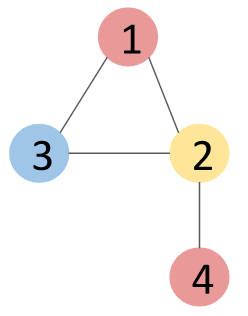
\includegraphics[height=3.8cm,width=3.2cm]{images/graphs/graph.png}
  \caption{Graph G}
  \label{C2H4-1}
\end{minipage}
\begin{minipage}[t]{.4\textwidth}
  \centering
  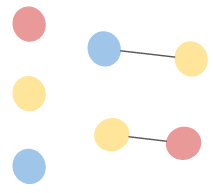
\includegraphics[height=3.3cm,width=3.5cm]{images/features.png}
  \caption{Paths of G of length less or equal to 1}
  \label{features}
\end{minipage}
\end{figure}
%%

\subsubsection{Implementation}
\label{pi:featuresImpl}
Algorithm \ref{alg:outputPath} describes the implementation of Steps 1-4 described above. Given a sequence of vertices \emph{p} as parameter, the procedure computes the \emph{p-feature} (line 2) and \emph{p-feature}$^{\prime}$ (lines 3, 4) and stores the lexicographically smaller variant in the index.

%%% proper output path algorithm
\begin{algorithm}
\centering
\caption{Compute p-features procedure}
\label{alg:outputPath}
\begin{algorithmic}[1]
\Procedure{computeFeature }{\emph{p}}
\State pfeature $\gets$ \emph{p}.toString() \Comment{\textit{returns a string of the labels of the nodes in vseq}}
\State \emph{revp} $\gets$ \emph{p}.reverse() \Comment{\textit{reverse the order of nodes in \emph{p}}}
\State pfeature$^{\prime}$ $\gets$ \emph{revp}.toString() \Comment{\textit{returns a string of the labels of the nodes in \emph{revp}}}
\If {pfeature$^{\prime}$ $<$ pfeature}
\State pfeature $\gets$ pfeature$^{\prime}$ \Comment{\textit{put to index the lexicographically smaller string}}
\EndIf
\If {pfeature $\notin$ $\fancyI_{D}$}
\State $\fancyI_{D}$ $\gets$ $\fancyI_{D}$ + pfeature %add pfeature to $\fancyI_{D}$
\EndIf
\EndProcedure
\end{algorithmic}
\end{algorithm}
%%% end of algorithm

\subsubsection{Candidates Extraction}
%for each path in the pattern index: check whether there exists the same path in the target index. Output the ids of all targets that contain all paths of the pattern.
Algorithm \ref{alg:piCandidatesExtraction} shows the candidates extraction procedure. It returns a list of the ids of all graphs in the database that contain all p-features of the pattern graph \emph{p}. Algorithm \ref{alg:piCandidatesExtraction} iterates once through all graphs in the \emph{D} (line 3) and for each target, checks whether its index contains all p-features of the pattern \emph{P} (lines 5, 6, 7). Let the size of the index of \emph{P} be $|\fancyI_{P}|$ on average and the average size of a target graph index be $|\fancyI_{T}|$. Then the time complexity is equal to $\mathcal{O}(|D|.|\fancyI_{P}|.|\fancyI_{T}|)$.

\begin{algorithm}
\centering
\caption{Candidates Extraction Procedure}
\label{alg:piCandidatesExtraction}
\begin{algorithmic}[1]
\Procedure{candidatesExtractor }{$\fancyI_{P}$, $\fancyI_{D}$}
\State{candidates $\gets$ new ArrayList$<>$()}
\For{ T $\in$ D}
	\State{flag $\gets$ true}
	\For{pfeature $\in$ $\fancyI_{P}$}
    	\If{ $\neg$\Call{contains }{ $\fancyI_{T}$, pfeature}} \Comment{\textit{check whether pfeature is contained in $\fancyI_{T}$}}
        	\State{flag $\gets$ false; break}
        \EndIf
	\EndFor
    \If{flag}
    	candidates $\gets$ candidates + T.id
    \EndIf
\EndFor
\State{\Return{candidates}}
\EndProcedure
\end{algorithmic}
\end{algorithm}

%%%%%%%%%%%%%%%%%%%%%%%%%%%%%%%%%
\subsection{Path-Subtree Index}
\label{path-subtree-index}
Path-Subtree Index (PSI) is a novel indexing technique based on the notion of vertex neighbourhood label, somewhat similar to the labeling approach used for solving the subgraph isomorphism problem, employed by \cite{Solnon:2010}. This Section presents the algorithm for computing the p-features of paths and the candidates extraction approach employed in PSI. We prove that PSI has greater filtering power than PI.

\subsubsection{Features}
The difference between PSI and PI lies in the algorithms that compute the unique string representation (p-feature) of paths. PSI uses an alternative labeling procedure, based on the \emph{neighbourhood label} (n-label) of a vertex. Below we discuss the notion of vertex neighbourhood label and the procedure of computing p-features.

\subsubsection{Vertex Neighbourhood Label}
The term \emph{neighborhood label (n-label)} refers to a specific label that is computed for each vertex in a graph \emph{G}, using the labels of the vertices in its neighbourhood. The n-label of a vertex \emph{v} with label \emph{l} is a string composed of the labels of its neighbours and \emph{l} ordered in lexicographically increasing order, starting always with \emph{l}.

%%%
\begin{figure}
\centering
\begin{minipage}[t]{.4\textwidth}
  \centering
  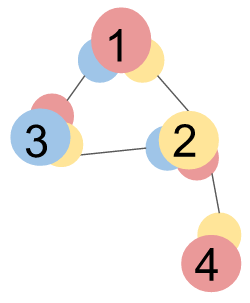
\includegraphics[height=4.4cm,width=3.7cm]{images/graphs/nlabels.png}
  \caption{Graph G with n-labels}
  \label{nlabels}
\end{minipage}
\begin{minipage}[t]{.4\textwidth}
  \centering
  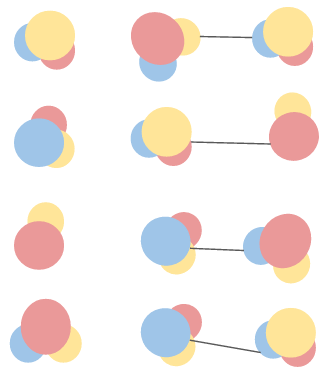
\includegraphics[height=4.8cm,width=4.2cm]{images/nfeatures.png}
  \caption{Paths of length less or equal to 1 with n-labels}
  \label{nfeatures}
\end{minipage}
\end{figure}
%%

%%% todo add the n-label images done for the presentation, change the example
\begin{example}
\label{ex:nlabel}
%Figure \ref{C2H4-1} represents a graph with 6 vertices with ids from 1 to 6. Each vertex is labeled either in yellow (Y) or in blue (B), as shown in the Figure. The n-label of vertex 6 is ``BBYYY'', as it is its label is B, it has 4 neighbours, 3 of them with label Y and one with label B. Similarly, the n-label of vertex 5 is ``BBY'', and the n-label of vertices 1, 2, 3 and 4 is equal to ``YB''.
Figure \ref{nlabels} shows the n-labels of the vertices in \emph{G} on Figure \ref{C2H4-1}. The n-label of each vertex starts with its own label, which is denoted in the picture as the biggest circle. For instance, the n-label of vertex 1 is composed of red (R), blue (B) and yellow (Y), starting with its own label, which is R, and then adding the labels of its neighbours (vertex 2 and 3). Note that although the n-labels of vertices 1, 2 and 3 contain the same colors, they are not the same. We write the n-label of vertex 1, 2 and 3 as ``RBY'', ``YBR'' and ``BRY'' respectively.
\end{example}

\begin{enumerate}
\item Given a sequence of vertices \emph{p}, replace each vertex in \emph{p} with its \emph{neighbourhood label (n-label)} to obtain the p-feature of \emph{p}.
\item Reverse \emph{p} to obtain \emph{p}$^{\prime}$.
\item Calculate \emph{p-feature}$^{\prime}$, that is the unique string representation of \emph{p}$^{\prime}$.
\item If not added previously, store in $\fancyI_{D}$ the lexicographically smaller of the two string representations (i.e. \emph{p-feature}$^{\prime}$ or \emph{p-feature}).
\end{enumerate}

\begin{example}
Figure \ref{nfeatures} shows all paths of length less or equal to 1, composed from \emph{G} with n-labels on its vertices on Figure \ref{nlabels}. The p-features stored in the index of \emph{G} consist of the lexicographically smaller variant of their string representation. For instance, the p-feature of the top-most right-most path is the string ``RBY-YBR''.
\end{example}

\subsubsection{Implementation}

The toString method used in Algorithm \ref{alg:outputPath} is modified to take a bit as an input, which constructs a p-feature using the n-labels of the vertices of the bit is set or returns a p-feature composed of the labels of the vertices otherwise.

One can see that the difference between the features representation and computation between PI and PSI lies only in Step 1. The algorithm to implement the features representation and storage is almost the same as the one for PI with (Algorithm \ref{alg:outputPath}). The only difference is the modification of the toString() method (line 2,4) to output the n-labels or the labels of the vertices in the sequence depending on the value of a bit given as an input parameter. The p-features are constructed using labels of vertices if the bit is set to false or using the n-labels otherwise. The n-labels of the vertices in each graph are computed prior to the invocation of Algorithm \ref{alg:outputPath}, as explained below. Thus there is no additional time complexity to the features representation and storage algorithm used in PI.

Computing the n-label of a vertex is done after all the graphs from the input files are read and initialized. Additional field called n-label of type String and methods to compute it are added to the Vertex class. Algorithm \ref{alg:nlabel} shows our approach. It is executed for every vertex in every target. For every vertex, we compute a sequence of labels of its neighbours ordered lexicographically. The complexity of insertion sort is $\mathcal{O}(n^{2})$ \cite{backtracking-algorithms} and therefore the overall complexity of running Algorithm \ref{alg:nlabel} is $\mathcal{O}(d.n^{2})$, where \emph{d} denotes the average degree of a vertex and \emph{n} is the size of the n-label, that is \emph{d+1}.
 
%%% n-label algorithm
\begin{algorithm}
\centering
\caption{Set n-label procedure}
\label{alg:nlabel}
\begin{algorithmic}[1]
\Procedure{setNlabel }{}
\State{nlabel $\gets$ initialize}
\For{Edge e $\in$ edges}
\State u $\gets$ e.dstVertex
\State \Call{insertionSort }{nlabel, u.label} \Comment{\textit{Insert u`s' label in n-label in lexicographically increasing order}}
\EndFor
\EndProcedure
\State{nlabel $\gets$ label + nlabel} \Comment{\textit{append the label of the vertex to its n-label}}
\end{algorithmic}
\end{algorithm}
%%% end of algorithm

\subsubsection{Candidates extraction}
\label{pi:candExtr}
This Section describes how the set of candidate graphs for a \gls{sip} test with the pattern is formed, using the database index $\fancyI_{D}$ and the set of features of the pattern $\fancyI_{P}$.

We say that a p-feature \emph{A}, composed by the n-labels of the vertices of a path \emph{a}, \emph{includes} a p-feature \emph{B}, composed by the n-labels of the vertices of a path \emph{b}, if the following conditions are met:
\begin{enumerate}
\item Every vertex \emph{v} in position \emph{i} in \emph{b}, has label equal to the label of a vertex \emph{w} in position \emph{i} in a.
\item The n-label of every vertex \emph{v} in position \emph{i} in \emph{b} is a substring of the n-label in position \emph{i} in \emph{a}.
\end{enumerate}

The method to extract the candidate set is the same as the one shown in Algorithm \ref{alg:piCandidatesExtraction}. The only change is in the implementation of the contains procedure (Algorithm \ref{alg:piCandidatesExtraction} line 6). Instead of checking whether there exists a feature in the target index $\fancyI_{T}$ that is identical to a given pattern feature \emph{pf}, we check whether there exists a p-feature in $\fancyI_{T}$ that includes \emph{pf}.

The first condition is equivalent to the filtering procedure employed by PI: we check for compatibility using only the labels. The purpose of the second condition is to verify that the neighbourhood of each pattern vertex can be matched to a neighbourhood of a vertex in the target.

Algorithm \ref{alg:psicandidatesExtraction} illustrates the implementation of the includes procedure. For every path in the target index, it calls Algorithm \ref{alg:psicontainsFeature} to check that the two conditions for the target p-feature to include the pattern p-feature are met (Algorithm \ref{alg:psicandidatesExtraction} line 3). If condition 1 (Algorithm \ref{alg:psicontainsFeature} line 2) is met, then procedure containsLabel checks whether condition 2 is satisfied (Algorithm \ref{alg:psicontainsFeature} line 8). Procedure isSubstring takes two nlabels as arguments and returns true if the second nlabel is a substring of the first nlabel or false otherwise.
%%% 
\begin{algorithm}
\centering
\caption{Includes procedure}
\label{alg:psicandidatesExtraction}
\begin{algorithmic}[1]
\Procedure{includes }{Tindex, patPath} \Comment{\textit{Tindex is the target index, patPath is path in the pattern index}}
\For{tarPath $\in$ Tindex}
	\If{\Call{includesFeature}{tarPath, patPath}}
    \State{\Return{true}}
    \EndIf
\EndFor
\State{\Return{false}}
\EndProcedure
\end{algorithmic}
\end{algorithm}

\begin{algorithm}
\centering
\caption{includesFeature procedure}
\label{alg:psicontainsFeature}
\begin{algorithmic}[1]
\Procedure{includesFeature}{tarPath, patPath}
\If{tarPath.length $<$ patPath.length} \Return{false} \Comment{\textit{if tarPath is shorter than patPath, then it can`t contain it}}
\EndIf
\If{label of each vertex in tarPath \textbf{not equal} label of each vertex in patPath} \Comment{\textit{equivalent to PI filter}}
	\State{\Return{false}}
\EndIf
\For{i in range(0, tarPath.length)} \Comment{\textit{for i$^{th}$ nlabel in tarf, check that it includes the i$^{th}$ nlabel in patPath}}
    \If{ $\neg$\Call{isSubstring}{tarPath[i], patPath[i]}}
        \State{\Return{false}}
    \EndIf
\EndFor
\State{\Return{true}}
\EndProcedure
\end{algorithmic}
\end{algorithm}

Algorithm \ref{alg:psicandidatesExtraction} involves visiting each path in the index of a single target, calling Algorithm \ref{alg:psicontainsFeature} (line 3), which then visits at most all characters that form a given nlabel. Therefore, the overall complexity of Algorithm \ref{alg:psicandidatesExtraction} is linear with the size of the input.

%%% WHY IS NEIGHBORHOOD METHOD BETTER? %%%
\begin{theorem}
\label{psiisbettertheorem}
Let $\fancyC_{PI}$ be the candidate set retrieved by PI and let $\fancyC_{PSI}$ be the candidate set obtained after running the framework using PSI. Then $\fancyC_{PSI}$ $\subseteq$ $\fancyC_{PI}$.
\end{theorem}

\begin{proof}
The necessary conditions for a p-feature \emph{A} to include a p-feature \emph{B} are the proof of the Theorem. The first condition puts an upper bound on the size of $\fancyC_{PSI}$ to be at most $|\fancyC_{PI}|$. The second condition gives PSI additional filtering strength by requiring an existence of matching of the neighbourhood of each pattern vertex to a neighbourhood of a vertex in the target. Therefore $\fancyC_{PSI}$ $\subseteq$ $\fancyC_{PI}$. 
\end{proof}

\section{Running the framework}
To run the framework, the user specifies the names of the files containing the database and the query set, \emph{k} (the bound on the path length allowed to be extracted) and a bit denoting which indexing and candidates extraction technique the user wants to run. If the bit is 1, the framework will index the graphs using PSI, otherwise it will run PI. The source code can be downloaded from Github \cite{framework-github}.

\section{Performance analysis and suggestions for improvement}
\label{sec:performance}
In this Section we discuss the performance of the framework using PI and PSI. Both of them were ran with the Aids dataset, described in Section \ref{sec:datasets}. Their filtering strength and execution time was compared with CT-Index \cite{ctindex}, analyzed in Section \ref{sec:ctindex}. CT-Index results are also used as a benchmark for correctness of the implemented algorithms. We outline the strengths and weaknesses of PI and PSI and give suggestions for improvement.
Let us denote the index and the candidate set obtained after running the framework using PI as $\fancyI_{PI}$ and $\fancyC_{PI}$ respectively, and the index and the candidate set obtained after running the framework using PSI as $\fancyI_{PSI}$ and $\fancyC_{PSI}$. 

PSI requires significantly more storage space than PI, due to the fact that it uses n-labels to encode features. The length of the n-label of a vertex is equal to its degree, incremented by 1. In particular, if we assume that the average vertex degree in the target database is \emph{d}, the p-feature of each path computed using PSI will be \emph{d} times bigger than the p-feature of the same path computed using PI due to the size of the nlabel of each vertex. Therefore, the size of $\fancyI_{PSI}$ is \emph{d} times bigger than the size of $\fancyI_{PI}$.

%% todo: write the number of real sat sip
\begin{table}
\renewcommand{\arraystretch}{1.2}
\parbox{.45\linewidth}{
\centering
\begin{tabular}{|c|r|r|r|}
\hline
  \emph{k} & \# candidates & running time & FP ratio\\
  \hline
  2 & 39,368 & 16,509 & 0.79 \\
  3 & 33,995 & 25,653 & 0.76 \\
  4 & 31,831 & 58,559 & 0.74 \\
  5 & 31,106 & 149,091 & 0.74 \\
 \hline
\end{tabular}
\caption{PI}\label{table:PI}
}
\parbox{.45\linewidth}{
\centering
\begin{tabular}{ |c|r|r|r|}
\hline
  \emph{k} & \# candidates & running time & FP ratio\\
  \hline
  2 & 17,863 & 25,662 & 0.54 \\
  3 & 9,363  & 71,099 & 0.14 \\
  4 & 8,336  & 228,992 & 0.03 \\
  5 & 8,240  & 731,450 & 0.02 \\
 \hline
\end{tabular}
\caption{PSI}\label{table:PSI}
}
\caption{Performance of PI and PSI depending on the maximum path length bound (\emph{k}). The number of SAT SIP instances of \emph{D} and \emph{Q} is 8,042}
\label{table:PIandPSI}
\end{table}
%%%

Consider Table \ref{table:PIandPSI} that shows the performance of the framework when run with PI (Table \ref{table:PI}) and PSI (Table \ref{table:PSI}). The data on the two tables is obtained after running the database \emph{D} with query \#0 from the query set \emph{Q}, where \emph{D} and \emph{Q} are from the Aids dataset. The size of \emph{D} is equal to 40,000 and the number of SAT SIP instances between pattern \#0 and \emph{D} is 8,042 \cite{datasets}. The first column of each table shows the maximum bound on the path length, \emph{k}, the second column denotes the number of candidates obtained for each \emph{k}, and the third column shows the framework running time. The fourth column shows the FP ratio for each \emph{k}, where the FP ratio is calculated using formula \ref{eq:fpratio}, discussed in Section \ref{subsec:ctindexEval}.

Note that the maximum value of \emph{k} is equal to 5. This is due to the fact that when \emph{k} is bigger than 5, the framework for PSI does not finish execution for hours. This follows from the complexity analysis of the algorithms that are implemented in the framework, which was carried out earlier. 

Theorem \ref{psiisbettertheorem} states that the filtering performance of PSI is not worse than the filtering performance of PI. Our experiments show that for the Aids dataset, the size of $\fancyC_{PSI}$ is rarely close to the size of $\fancyC_{PI}$. Comparing the second column of Table \ref{table:PI} with the second column of Table \ref{table:PSI}, one can see that $\fancyC_{PI}$ is more than twice bigger than $\fancyC_{PSI}$ for each \emph{k}. The increase of \emph{k} increases the difference between the size of $\fancyC_{PI}$ and $\fancyC_{PSI}$, and when \emph{k} equals 5, PSI prunes 31,760 targets and $\fancyC_{PSI}$ contains only 198 false-positives. This shows that n-labels manage to capture substantially more information about the structure of the graphs and lead to several times better filtering performance.

It is interesting to observe that the difference of the size of $\fancyC_{PSI}$ is very small for \emph{k} equal to 4 and 5 (Table \ref{table:PSI}). However, the running time of PSI for \emph{k} = 5 is 3 times bigger than the running time of PSI for \emph{k} = 4. This suggests that the filtering power does not increase linearly with the running time with increasing \emph{k} and there exists a maximum value of \emph{k} = $\lambda$, when the trade off between filtering power and running time is good. Then, for \emph{k} $>$ $\lambda$, there is almost no filtering gain, but only significantly increased computation and storage overhead. Similar observation can be made for PI (Table \ref{table:PI}).

PSI is several times slower than PI. Comparing the third column of Table \ref{table:PI} with the third column of Table \ref{table:PSI}, one can see that for each \emph{k}, the running time of PI is much better than the running time of PSI. Their difference increases with increasing \emph{k}. There are several reasons for these results. One of them is that the size of $\fancyI_{PI}$ is several times smaller than the size of $\fancyI_{PSI}$. The size of the index plays major role in the complexity of the candidates extraction procedure for both PI and PSI, as shown previously. A second reason is that computing the n-labels of the vertices of each graph requires additional running time.

%Both PI and PSI are much slower than CT-Index. In particular, increasing the maximum path length bound significantly increases the algorithms computation time. This stems from the fact that maximum path length makes great impact on the complexity of the path extraction algorithm and on the size of the index. PSI is slower than PI both during index computation and candidates extraction time. Looking at the difference in their time complexities, this result is not surprising.

%The filtering power of PSI and PI does increase linearly when increasing the maximum path length bound. There exists a bound \emph{m} on the maximum path length after which there is almost no filtering gain, but only significantly increased computation and storage overhead. The value of \emph{m} is usually smaller for PSI than for PI. For instance, when PSI is ran with instances from the AIDS dataset, \emph{m} is equal to 5. This is the peak when the algorithm performs best. Any value larger than 5 results in much worse computation speed and almost unchanged filtering performance.

The performance results show that the framework has slow running time that makes it hard to be used in practice. However, they also show that PSI has very strong filtering capability. Below, we suggest possible techniques for running time improvement of the framework.

The index of the database is represented as the union of the indices of all targets. Naively, it does not take into an account the fact that a feature can be present in more than one graph. When working with datasets where the graphs are similarly structured like Aids, removing repetitive features results in significant decrease of the index size. The following strategies can be employed to decrease the size of the index without lowering its filtering capability.

We can represent the index using a \gls{tree} data structure similar to \gls{sufftree} \cite{weiner:1973} that stores all extracted features from the database as strings and number of leaf nodes of the tree denotes the number of features. The representation of strings in the tree is the same as the representation employed by \glspl{sufftree} except from the construction of leaf nodes and the feature suffixes insertion. Each leaf node is a list of the ids of all graphs that contain the corresponding feature. We insert the full feature without inserting its suffixes. This is because each label/nlabel part of a feature is a feature on its own and it will be extracted from the path extraction algorithm. Therefore, there is no need to insert unique termination character at the end of a feature, as it is done with \glspl{sufftree}. The tree can be built incrementally during features extraction in $\mathcal{O}(n.log(n))$ time on average, where \emph{n} is the length of the string that results when appending all features in the database, and worst-case time complexity $\mathcal{O}(n^{2})$. More efficient suffix tree construction algorithms exist \cite{weiner:1973, McCreight:1976, Ukkonen:1995} that could be adjusted to work for the tree. Searching for a feature \emph{F} of length \emph{m} in the suffix tree requires following a path from the root matching characters until reaching the leaf node and can be done in $\mathcal{0}(m)$ time. %Therefore, candidates extraction with pattern index with \emph{n$_{p}$} number of features of average length \emph{m$_{p}$} and target index with \emph{n$_{d}$} number of features of average length \emph{m$_{d}$} would take $\mathcal{O}(n)$ has time complexity $\mathcal{O}()$

%Alternative way is to represent the index as a dictionary. - having a dictionary structure to keep every feature and the number of times it occurs in the particular graph. Analyze what the complexity of this would be, would it be better and why.

%- the framework provides a functionality to save the index to a file and then reuse it from the file. In practice, the way the code works at the moment is to store the target index in memory. Experiments with the datasets used by big data research community were run on a simple machine and no memory overflow was encountered.

%- reduce the index size by employing the maximal features thing (cite needed papers --- graphgrepsx about the idea and the early IBM paper about the notion of descriptive feature).

% TODO: write that we can represent the graphs using bitset encodings. cite the papers cited by patrick and ciaran's sip paper.

%%%%%%%%%%%%%%%%%%%%%%%%%%%%%%%%%%%%%%%%%%%%%%%%%%%%%%%%%%%%%%%%%%%%%%%%%%%%
%%%------------------------------SIP Algorithms--------------------------%%%
%%%%%%%%%%%%%%%%%%%%%%%%%%%%%%%%%%%%%%%%%%%%%%%%%%%%%%%%%%%%%%%%%%%%%%%%%%%%

%% todo
%% remove sip0 and make sip1 be sip 0
%% make the graphs be in log scale
\chapter{Light Filters}
\label{ch:sip1}
This section describes the study of a simple subgraph isomorphism problem(\gls{sip}) algorithm, called SIP1, that implements a fast filter that does not employ an index structure.

Light Filters is an algorithm for subgraph query processing that is based on a modified version of the filter-verification paradigm. This approach uses simple filtering tests that require much less computational effort. 
Given a database \emph{D} and a query set \emph{Q}, subgraph query processing for \emph{D} and \emph{Q} takes every instance, executes filtering procedures, and if the instance is not proved as (unsatisfiable) \gls{unsat}, a subgraph isomorphism problem (SIP) test is called to solve it. Unlike classical filtering-verification model, no candidate set is computed, because if a target \emph{T} is candidate for a pattern \emph{P}, SIP is carried out immediately. Additionally, here more importance is placed on the quality of the \gls{sip} algorithm. 

Algorithm \ref{algo:roughSIP} gives an outline of our approach. We first read in each graph in \emph{D} and \emph{Q} and initialize graph objects (lines 2, 3). Filtering is performed for every (\emph{P}, \emph{T}) pair,  and if the instance is not pruned, a call to a \gls{sip} algorithm is made (line 7). The filtering step consists of 5 simple tests, performed before the call to SIP1. If the conditions of any of the tests are not met, search does not proceed, we call this a \emph{trivial fail} and carry on with the next instance. 

The remaining of this Chapter gives an explanation of each step of the Light Filters algorithm. First, we introduce the theory behind the trivial failures and their implementation in Section \ref{sec:trivialFails}. We then introduce the subgraphs isomorphism problem algorithm called SIP1 and discuss its implementation in Section \ref{sec:sip1}. We give an empirical analysis of each of the algorithms implemented in our subgraph query processing approach. Evaluation of Light Filters and discussion of our experimental results is described in the next Chapter.

%%% light filters sip algorithm
\begin{algorithm}
\centering
\caption{Light filters algorithm}
\label{algo:roughSIP}
\begin{algorithmic}[1]
\Procedure{Compute }{\emph{Q}, \emph{D}}
\State targets $\gets$ read in all targets from \emph{D}, initialize objects
\State patterns $\gets$ read in all patterns from \emph{Q}, initialize objects
\For{P $\in$ patterns}
	\For{T $\in$ targets}
		\If{!\Call{Filter }{P, T}} \Comment{\textit{If the instance is not rejected during filtering, perform verification}}
    		\State{\Call{SIP1}{P, T}}
    	\EndIf
    \EndFor
\EndFor
\EndProcedure
\end{algorithmic}
\end{algorithm}
%%%% end of algorithm

\section{Trivial Failures}
\label{sec:trivialFails}

This Section introduces the five trivial failure tests, implemented as part of the filtering stage of SIP1. The tests are based on the notion of neighbourhood degree sequence, a concept also used in \cite{Solnon:2010}. First, we introduce definitions and notations that complement the theory section in Chapter \ref{ch:introduction}. We then prove the correctness of our approach and outline its implementation and give an empirical analysis of each of the tests.

The \emph{label neighbourhood degree sequence} (LNDS) of label \emph{l} in L(\emph{G}) for a graph \emph{G}, denoted as LNDS (\emph{G}, \emph{l}) is the sequence of the degrees of all vertices in \emph{G} that have \emph{l} assigned as their label, taken in non-increasing order.

%Let \emph{A} and \emph{B} be sequences of integers. We say that \emph{B} is a \emph{subsequence} of \emph{A} if \emph{B} can be derived from \emph{A} by deleting zero or more elements in \emph{A}. An element of a sequence \emph{A} at index \emph{i} is the \emph{i}-th element of \emph{A}, denoted by \emph{A$_{i}$}. 

We say that \emph{A} \emph{subsumes} \emph{B}, \emph{A} $\succeq$ \emph{B}, if there exists a subsequence \emph{A$^\prime$} of \emph{A} with length equal to the length of \emph{B}, such that \emph{B$_{i}$} is less than or equal to \emph{A$_{i}^\prime$} for all indices \emph{i} for \emph{A$^\prime$}, \emph{B}.

\begin{example}
Let \emph{A} be the sequence of integers \{4, 3, 2\} and let \emph{B} be the sequence of integers \{2, 2\}. Then, \emph{A} $\succeq$ \emph{B} and an example of sequence \emph{A$^\prime$} from the definition is \{4, 3\}.
\end{example}

\begin{figure}
\centering
\begin{minipage}[t]{.3\textwidth}
  \centering
  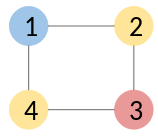
\includegraphics[height=2.1cm,width=2.3cm]{images/graphs/exampleGraph2.png}
  \caption{graph P}
  \label{fig:P}
\end{minipage}%
\begin{minipage}[t]{.4\textwidth}
  \centering
  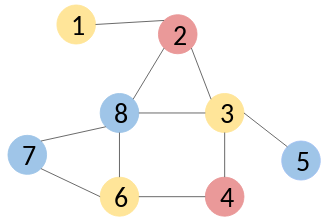
\includegraphics[height=3.4cm,width=5cm]{images/graphs/exampleGraph.png}
  \caption{graph T}
  \label{fig:T}
\end{minipage}
\caption{Instances of subgraph isomorphism problem (SIP)}
\label{fig:lightFiltersExample}
\end{figure}

By abuse of notation, we say that a graph \emph{T} \emph{subsumes} a graph \emph{P}, \emph{T} $\succeq$ \emph{P}, if for every label \emph{l} in \emph{P}, LNDS (\emph{T}, \emph{l}) $\succeq$ LNDS (\emph{P}, \emph{l}).

\begin{example}
Let us look at graphs \emph{T} and \emph{P} on Figure \ref{fig:lightFiltersExample}. Both of them consist of three labels: yellow (Y), red (R) and blue (B). Let us compute LNDS of every label in \emph{T} and \emph{P}. LNDS (\emph{T}, Y) = \{4, 3, 1\}, LNDS (\emph{T}, R) = \{3, 2\} and LNDS (\emph{T}, B) = \{4, 2, 1\}. Similarly, LNDS (\emph{P}, Y) = \{2, 2\}, LNDS (\emph{P}, R) = \{2\} and LNDS (\emph{P}, B) = \{2\}. Clearly, \emph{T} subsumes \emph{P}, as for every label \emph{l} in \emph{P}, LNDS (\emph{T}, \emph{l}) $\succeq$ LNDS (\emph{P}, \emph{l}).
\end{example}

Let $\Lagr$ be the labeling function in \emph{G} and let us define a label counting function for \emph{G}, $\lambda_{G}$ : $\Lagr$ $\rightarrow$ $\mathbb{N}$ as follows:
for any \emph{l} $\in$ $\Lagr$ if there is no vertex in \emph{G} with label \emph{l}, $\lambda_{G}$(\emph{l}) = 0. Otherwise $\lambda_{G}$(\emph{l}) is equal to $|L^{-1}(l)|$, that is the number of vertices in \emph{G} which are assigned \emph{l} as their label.

\begin{example}
Let us consider graph \emph{P} in Figure \ref{fig:P} that is assigned three labels: red (R), yellow (Y) and blue (B). The counting function of each of them is the following: $\lambda_{P}$(R) = 1, $\lambda_{P}$(Y) = 2 and $\lambda_{P}$(B) = 1.
\end{example}

We can now introduce several simple filtering tests for incompatibility between graphs \emph{P} and \emph{T}. If either of the tests is not true, \emph{P} is not subgraph isomorphic to \emph{T} and we say that we have encountered a \emph{trivial fail}. If an instance causes a trivial fail, we do not have to test for subgraph isomorphism, because in such case this instance is UNSAT. The filtering tests are shown on Figure \ref{table:failures}. Their execution follows a strict hierarchy based on the expected cost of their execution, starting with the test which is shown to require least computational effort (test 1). Analysis of the complexity of each test is given later in this Section. Every test is executed only if all previous tests succeeded. Below follows a proof of the correctness of first four filtering tests. The fifth test is discussed shortly. 

%%%% table about failures %%%%
\begin{table}[H]
\centering
\renewcommand{\arraystretch}{1.5}% Spread rows out...
\begin{tabular}{ >{\centering\bfseries}m{1in} >{\centering\arraybackslash}m{2.3in}} 
\toprule
  Trivial Fail & Meaning\\
\midrule
 \textbf{1} & $|V (T)|$ $\geq$ $|V (P)|$\\
 \rowcolor{Gray}
 \textbf{2} & $|L(V(\emph{T}))|$ $\geq$ $|L(V(\emph{P}))|$\\
 \textbf{3} & $\forall$ \emph{l} $\in$ $\Lagr$: $\lambda_{P}(l)$ $\leq$ $\lambda_{T}(l)$\\
 \rowcolor{Gray}
 \textbf{4} & \emph{T} $\succeq$ \emph{P}\\
 \textbf{5} & $\forall$ \emph{v} $\in$ V(\emph{P}), domv $\neg$  $\varnothing$\\
 \bottomrule
\end{tabular}
\caption{Failure tests hierarchy}
\label{table:failures}
\end{table}        
%%%%

\begin{theorem}
\label{th:nds}
Let \emph{T} and \emph{P} be graphs. If either of the following failure tests:
\begin{enumerate}
\item \label{test1} $|V(T)|$ $\leq$ $|V(P)|$
\item \label{test2} $|L(V(T))|$ $\leq$ $|L(V(P))|$
\item \label{test3} T $\succeq$ P
\item \label{test4} $\forall$ \emph{l} $\in$ $\Lagr$: $\lambda_{P}(l)$ $\leq$ $\lambda_{T}(l)$
\end{enumerate}
is false, then \emph{P} is not subgraph-isomorphic to \emph{T}.
\end{theorem}

\begin{proof}
By contradiction. Suppose that \gls{sip} (\emph{P}, \emph{T}) is \gls{sat}.

Suppose that test \ref{test1} is false. Then, \emph{P} must have at least one vertex more than \emph{T}, which means that this vertex would be unmatched. Therefore, from the definition of subgraph isomorphism, no valid mapping from \emph{P} to \emph{T} exists. Test \ref{test1} must be true.

Suppose that test \ref{test2} is false so that there exists a label \emph{l} in L(\emph{P}) that does not belong to L(\emph{T}). Therefore, there exists a vertex \emph{v} in \emph{P} with label \emph{l} that would be left unmatched.  Therefore, from the definition of subgraph isomorphism, \emph{P} is not isomorphic to \emph{T}. Test \ref{test2} must hold.

Suppose that test \ref{test3} is false and there exists a label \emph{l} both in L(\emph{P}) and L(\emph{T}) that is assigned to \emph{m} number of vertices in V(\emph{T}) and to at least \emph{m + 1} vertices in V(\emph{P}). That means that either at least one pattern vertex would be left unmatched, or at least two pattern vertices would be matched to the same target vertex. Either of these cases would violate the necessary conditions for \emph{P} to be subgraph isomorphic to \emph{T}. This is a contradiction, therefore test \ref{test3} must hold.

Suppose that \emph{T} does not subsume \emph{P}. Therefore, there exists label \emph{l} both in \emph{P} and \emph{T} such that LNDS (\emph{T}, \emph{l}) $\npreceq$ LNDS (\emph{P}, \emph{l}). From the proof that the previous three conditions must hold, it follows that LNDS (\emph{T}, \emph{l}) $\npreceq$ LNDS (\emph{P}, \emph{l}), because there exists at least one vertex \emph{v} whose degree is in LNDS (\emph{P}, \emph{l}) with higher degree than the degree of the corresponding vertex  in LNDS (\emph{T}, \emph{l}). A matching, of \emph{v} a vertex in V(\emph{T}) that preserves adjacency does not exists and \emph{P} is not subgraph isomorphic to \emph{T}, which is a contradiction. Test \ref{test4} must be true. 

We can deduce that if \emph{P} is subgraph isomorphic to \emph{T}, then each of the first four trivial tests must hold. From the rules of classical logic it follows that if either of the tests is false, then \emph{P} is not subgraph isomorphic to \emph{T}.
\end{proof}

The fifth trivial failure test is based on the choice of model for our subgraph isomorphism algorithm (SIP1). Given a pattern \emph{P} and a target \emph{T}, we represent each vertex \emph{v} in V(\emph{P}) as a variable that can accept one of the vertices in V(\emph{T}) as a value. The set of all possible values of \emph{v} is called the \emph{domain} of \emph{v}, \emph{domv}. It is represented as a bit array (bitset) of size equal to the order of \emph{T}, where each entry maps to a target vertex. domv[i] is equal to 1 if \emph{v} can be mapped to the i$^{th}$ vertex in V(\emph{T}), or 0 otherwise. If every bit in domv is 0, this means that no valid mapping from \emph{v} to any vertex in V(\emph{T}) exists. In such case \emph{v} has a \emph{domain wipe out}. During search, domain wipe out of \emph{v} indicates that the current partial mapping can not be a subgraph isomorphism from \emph{P} to \emph{T}. During initialization, domain wipe out of \emph{v} indicates that \emph{P} is not subgraph isomorphic to \emph{T}. Test 5 checks whether domv experiences a domain wipe out. If there exists an empty domain, the test fails and the instance does not proceed to search.
%% todo wirte that domain wipeout is a common test

\subsection{Implementation and complexity analysis}
\label{sec:trivialFailsImplementation}
Algorithm \ref{algo:filters} describes the implementation of the 5 trivial failures from Table \ref{table:failures} as part of the filtering stage. If any of the if statements (lines 2, 4, 7, 10 and 21) is false, the procedure returns false and verification is not executed. Otherwise, if all 5 tests are true, the procedure makes a call to SIP1 (Algorithm \ref{algo:sip1}), which is discussed in the next Section.

%% comment on the expensiveness of each trivial failure
Now follows a discussion about the cost of each failure test.
Failures 1 and 2 are the fastest: each of them takes $\mathcal{O}(1)$ time to compute. For failure 1, one needs only to return the sizes of the number of vertices in \emph{P} and in \emph{T}, which is computed while initializing the graphs. For failure 2, for every graph \emph{G}, we have an array that stores all unique labels that occur in \emph{G}. The size of this array is known after the initialization of \emph{G}. To check whether test 2 is true, one needs to compare the size of the labels array of \emph{P} with the size of the labels array of \emph{T},  which takes $\mathcal{O}(1)$ time.

%% todo there is something wrong on lines 4, 5 here
Failures 3 and 4 have slower running time. Checking whether $\lambda_{P}(l)$ is bigger than $\lambda_{T}(l)$ involves iterating over all labels in L(V(\emph{P})), and for each of them checking $\lambda_{T}(l)$, which can be found in constant time by taking the size of the pre-computed LNDS(\emph{T}, \emph{l}). Therefore, the overall complexity of failure 3 is $\mathcal{O}(|L(V(\emph{P}))|)$. Algorithm \ref{algo:subsumes} shows the pseudo code of the fourth failure test, called in line 10 in Algorithm \ref{algo:filters}. Test 4 iterates over the LNDS of every label \emph{l} in L(V(\emph{P})) and checks whether LNDS (\emph{T}, \emph{l}) $\succeq$ LNDS (\emph{P}, \emph{l}) (lines 5, 6). The correctness of the implementation follows from the fact that the elements in LNDS are ordered in non-increasing order. The complexity of test 4 is therefore $\mathcal{O}$($|$L(V(\emph{P}))$|.|$LNDS (\emph{T}, \emph{l})$|$).

Failure 5 visits each vertex \emph{v} in V(\emph{P}) (line 13), initializes domv (line 14) and for every \emph{w} in V(\emph{T}), checks whether \emph{w} can be mapped to \emph{v} (lines 15, 16). The complexity of this test is therefore equal to $\mathcal{O}(|V(P)|.|V(T)|)$.
%% failures algorithm
\begin{algorithm}
\centering
\caption{Lights Filters}
\label{algo:filters}
\begin{algorithmic}[1]
\Procedure{Filter }{G$_{p}$, G$_{t}$}
\If {$\neg$ $|V(T)|$ $\geq$ $|V(P)|$} \Return false \Comment{\textit{trivial failure 1}}
\EndIf
\If {$\neg$ $|L(V(T))|$ $\geq$ $|L(V(P))|$} \Return false \Comment{\textit{trivial failure 2}}
\EndIf
\For {\textit{l} $\in$ $|L(V(P))|$} %% todo write it with lambda
	\If {$\lambda_{P}(l)$ $>$ $\lambda_{T}(l)$} \Return false \EndIf \Comment{\textit{trivial failure 3}}
\EndFor
\If {$\neg$\Call{subsumes }{T, P}} \Return false \EndIf \Comment{\textit{trivial failure 4}}
\State alldoms $\gets$ initialize \Comment{\textit{An array of size the order of G$_{p}$ that contains the domain of each vertex in P}}
\For{every \textit{v} $\in$ V(\emph{P})}
\State{
	domv $\gets$ new BitSet($|V(T)|$) \Comment{\textit{initialize domV to bitset of size the order of the target}}
	\For{$\forall$ \textit{w} $\in$ V(\emph{T})}
    	\If {L(P, \emph{v}) = L(T, \emph{w}) $\land$ \textit{v}.degree $\leq$ \textit{w}.degree}
        \State {domv[\textit{w}] $\gets$ 1}
        \EndIf
	\EndFor
    \State {alldoms[v] $\gets$ domv}
	\If {domv = $\varnothing$} \Return false \Comment{\textit{trivial failure 5}}
}
\EndFor \\
\Call{sip1}{alldoms} \Comment{\textit{if no failures occurred, call SIP1 algorithm}}
\EndProcedure
\end{algorithmic}
\end{algorithm}
%%% end of algorithm

%%% subsumes
\begin{algorithm}
\centering
\caption{Graph T subsumes graph P}
\label{algo:subsumes}
\begin{algorithmic}[1]
\Procedure{subsumes }{T, P}
\For {\textit{l} $\in$ $|L(V(P))|$} %% todo write it with lambda
	\State{B $\gets$ LNDS (P, \emph{l})}
    \State{A $\gets$ LNDS (T, \emph{l})}
    \For{i in range (0, $|A|$)}
		\If {B[i] $>$ A[i]} \Return false
		\EndIf
	\EndFor
\EndFor \\
\Return true
\EndProcedure
\end{algorithmic}
\end{algorithm}
%%% end of subsumes
For the implementation of the filtering, the following classes are introduced.

\begin{itemize}
\item Class \emph{Graph}
It creates graph objects, given a file with graphs represented in a certain format. A graph object \emph{G} has size, denoted as \emph{m}, order, denoted as \emph{n}, \emph{id}, array of the degree of each vertex, called \emph{deg}, bitset array of the neighbours of each vertex, called \emph{N}, and array, called \emph{labels}, that stores all labels assigned to vertices in \emph{G}. \emph{N}$_{i}$ contains a bitset of the neighbours of the i-th vertex in \emph{G} and \emph{labels}$_{i}$ contains the label of the i-th vertex in \emph{G}, for every i between 0 and \emph{n}. Initialization of each of the aforementioned properties takes $\mathcal{O}$(m + n) time. When \emph{labels} is constructed, a new object for each unique label \emph{l} is created and LNDS (\emph{G}, \emph{l}) is computed.

\item Class \emph{Label}
This class represents a label \emph{l} in \emph{G}. \emph{l} has a \emph{name}, and an array of integers, sorted in non-increasing order that represents LNDS (\emph{G}, \emph{l}). It is built using insertion sort algorithm which is of complexity $\mathcal{O}(|LNDS (\emph{G}, \emph{l})|^{2})$ \cite{Cormen:2001:IA:580470}.

\item Class \emph{SIP1}
This class implements the light filtering procedure displayed in Algorithm \ref{algo:filters} as well as the \gls{sip} algorithm, which is explained in more detail in the next Section.
\end{itemize}

\section{SIP1 Implementation}
\label{sec:sip1}
SIP1 is a subgraph isomorphism algorithm, based on the simplest of the Glasgow algorithms \cite{CP2015}. Algorithm \ref{algo:sip1} shows a pseudocode of SIP1. It takes the domains of all vertices in the pattern \emph{P}, initialized in Algorithm \ref{algo:filters}), and repeatedly tries to assign to each variable (pattern vertex) a value (target vertex). If current assignment is compatible with the partial solution, the algorithm makes a recursive call (line 19) otherwise it backtracks. When a pattern variable \emph{u} is instantiated with a target value \emph{i} (line 9), all uninstatiated (future) variables have \emph{i} removed from their domains (line 12). If a future variable \emph{v} is adjacent to \emph{u} in \emph{P} then domv becomes the intersection of domv with the neighborhood of vertex \emph{i} in \emph{T}. This constraint is enforced by applying a logical \emph{and} operation between the two bit sets (line 14). SIP1 uses \gls{forwcheck} with fail first heuristic \cite{haralickElliot:1980}: for all uninstantiated variables representing pattern vertices, it selects to explore the one that has the smallest domain before the others (line 4).

%%% SIP1 pseudocode
\begin{algorithm}
\centering
\caption{SIP1 }
\label{algo:sip1}
\begin{algorithmic}[1]
\Procedure{SIP1 }{alldoms}
\If{alldoms = $\varnothing$} \Return solution \Comment{\textit{solution is either true or false}}
\EndIf
\State domu $\gets$ smallest(alldoms) \Comment{\textit{select vertex u with the smallest domain first}}
\State consistent $\gets$ false
\State newAlldoms $\gets$ initialize with size = ($|$alldoms$|$ - 1)
\For{i $\in$ domu.nextSetBit $\land$ $\neg$consistent} \Comment{\textit{for each entry in position i that could be assigned to u}}
	\State consistent $\gets$ true
	\State u $\gets$ i \Comment{\textit{assign i as a value of vertex u}}
	\For{(domv $\in$ alldoms) $\land$ (domv $\neg$= domu) $\land$ consistent} \Comment{\textit{iterate through the domain of each vertex while the current assignment is consistent}}
        \State newdomv $\gets$ domv
        \State newdomv[i] $\gets$ 0 \Comment{\textit{cannot take value assigned to u}}
        \If{(u, v) $\in$ E(\emph{P})} \Comment{\textit{If u is adjacent to v in \emph{P}}}
        	\State newdomv $\land$ neighbours of i $\in$ \emph{T} \Comment{\textit{v can only take vertices in G$_{t}$ adjacent to i}}
        \EndIf
        \State newAlldoms $\gets$ newAlldoms + newdomv \Comment{\textit{add newdomv to newAlldoms}}
        \State consistent $\gets$ (newdomv = 1) \Comment{\textit{if there is a domain wipe out, consistent becomes false}}
	\EndFor
    \State consistent $\gets$ consistent $\land$ \Call{SIP1}{newAlldoms} \Comment{\textit{call SIP1 if current assignment is consistent}}
\EndFor
\State \Return consistent
\EndProcedure
\end{algorithmic}
\end{algorithm}
%%% end of SIP1 pseudocode
In the worst case, SIP1 will assign all values from the domain of each pattern vertex, making recursive calls to SIP1 and failing late, therefore exploring very deep in the search tree before finding that there is no solution. In practice, due to the fail first heuristic used, the algorithm very rarely fails deep in the search tree, because the value that is most likely to fail is first explored, therefore failures occur mostly near the top of the search tree. 

\chapter{Evaluation}
\label{ch:evaluation}

This Section reports on the observed performance of the Light Filters subgraph query processing approach, described in Chapter \ref{ch:sip1}. Light Filters algorithm was run with each of the Big Data datasets, discussed in Section \ref{sec:datasets}, some of which were also used for experiments by \cite{foteini, graphgrepsx, GRAPES, graphgrepsx, ctindex, gcode, tree+delta>=graph, lindex}. Our experiments are conducted on a Windows 7 SP1 host with 2 Intel Xeon E5-2660 CPUs (2.20GHz, 20MB Cache, 8 cores/16 threads per CPU) and 128GB of RAM, which is the same machine used by \cite{foteini}. Run time is measured in milliseconds from when the process starts until it completes, including the time to read in all the graphs, to perform filtering and verification for each instance and to write out all results to a file.
% todo: write about the organisation of this chapter and write that evaluation of the framework is not done, but only empirical analysis

\section{Filtering performance}
\label{sec:sip1filterseval}
%% todo: write about what is said in this section
This Section reports our investigation of the quality of the filtering methods of Light Filters. Figure \ref{averageFailures} shows our results obtained for each of the four datasets.

The plot on Figure \ref{averageFailures} shows the following 7 metrics: the percentage of SAT instances (SAT SIP), the percentage of UNSAT instances that were discovered after verification (UNSAT SIP), and the percentage of instances that were discovered as UNSAT by failing one of the filtering tests (Fail 1, Fail2, etc.), following the same order as the one indicated in Table \ref{table:failures}, for each dataset.

The Figure shows four separate bars and a table with 5 columns and 7 rows. Each bar represents the 7 aforementioned metrics for one of the datasets. For instance, the leftmost bar represents results obtained from Aids and the rightmost- the results obtained from Ppigo. The color notation of each metric is given in the first column of the table. For example, the dark-most color shows SAT SIP and the white color represents Fail 1 for a given dataset.
Each table column under a given bar contains the same figures for the same dataset as the ones shown on the bar. They are supplied in order to help the reader see easier the exact value of each metric.

For instance, the leftmost bar represents Aids, where 8.67\% of all instances are \gls{sat}. Out of the \gls{unsat} problems, 24.211\% were discovered during the verification stage and the rest were filtered by either of the trivial failures. The number of \gls{sat} and \gls{unsat} problems is also given on Table \ref{table:dataSAT}.

Note that all SAT instances had to go through verification as well as all UNSAT instances that were not pruned during filtering (UNSAT SIP). For instance, for Aids, the total percentage of instances that were solved by call to SIP1 is 32.881\% and the rest of them were pruned by the failure tests. Looking at Figure \ref{averageFailures}, we make the following observations:

\begin{itemize}
\item Filtering gives best performance for the instances of Aids. In particular, 67.119\% of the targets are rejected before verification. A perfect filtering technique would prune additional 24.211\% of all instances in the dataset (UNSAT SIP).

\item Aids contains the largest number of \gls{unsat} instances (91.33\%), which means that a filtering algorithm has the chance to influence the performance of subgraph query processing for up to 91.33\% of all instances. Also, during analysis of existing work we observed that this dataset tends to be the main one (and sometimes the only one) used for evaluation for some subgraph query processing algorithms like \cite{graphgrepsx, ctindex, gcode, tree+delta>=graph}.

\item Filtering is not successful for any instance in Pdbs. In other words, verification was performed for every pattern and target in the dataset, as none of the instances was pruned by any of the failure tests. Similarly, only 3.75\% of the targets were filtered in Ppigo. Most of the instances of Pdbs and Ppigo are \gls{sat} (77.22\% and 61\% respectively) and they had to go through verification to be solved. Here, a perfect filtering technique would filter no more than 22.78\% and 39\% of the instances Pdbs and Ppigo respectively. In such cases, a subgraph query processing method that puts low effort in filtering and implements an efficient verification algorithm will have much higher performance than a method that employs heavy filtering approach and naive \gls{sip} algorithm for verification. This hypothesis is confirmed by the results of the study presented in \cite{foteini}, where some of the evaluated indexing techniques, considered as state of the art, never terminate for Pcms and Ppigo. This was also noted during the performance analysis of CT-Index in Section \ref{subsec:ctindexEval}.

\item There are duplicate target graphs in the Pcms and Pdbs. For instance, Pcms is supposed to contain 200 targets \cite{datasets}. In practice, there are only 50 unique graphs and each of them is added 4 times. Pdbs is composed of 600 targets \cite{datasets}, but out of them only 30 are unique, each of them duplicated 20 times.

\end{itemize}

One of the main points made above identifies the existence of a maximum bound on the effectiveness of all filtering techniques, that is the number of UNSAT instances for the given dataset. Unlike filtering, verification does not have such effectiveness limits.
 
%%% 
\begin{figure}
\centering
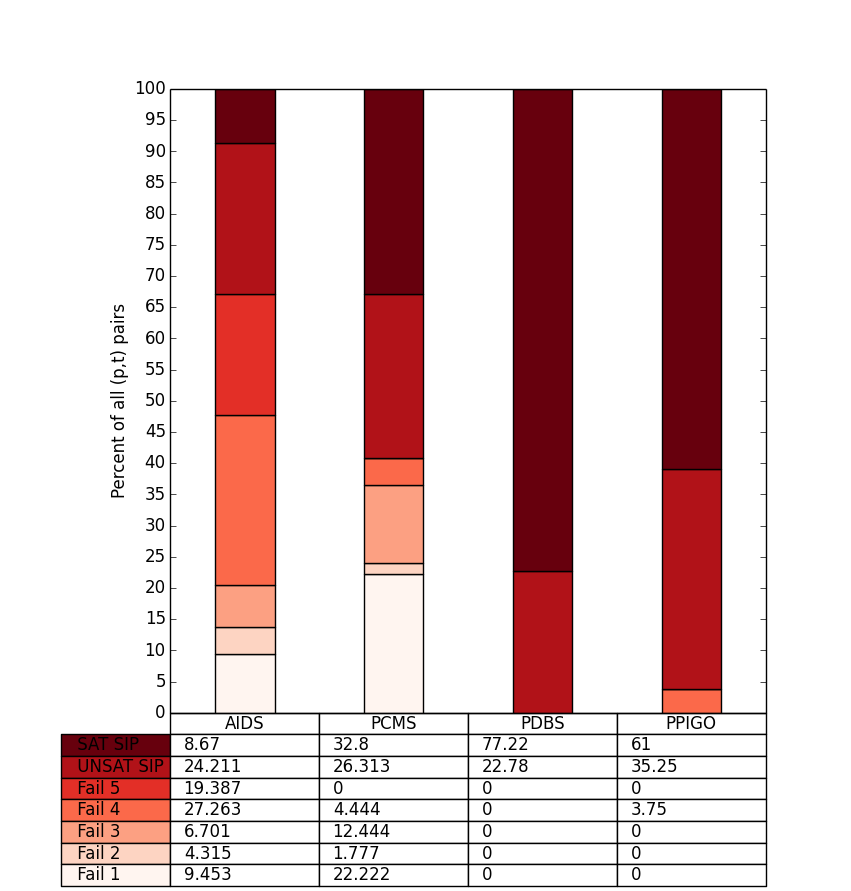
\includegraphics[height=15cm,width=13.5cm]{images/plots/splittedSIP.png}
\caption{Satisifability and average filtering percentage for each method in Table \ref{table:failures} for each of the datasets}
\label{averageFailures}
\end{figure}
%%%

\section{Hardness of verification}
In \cite{foteini} it is said that subgraph isomorphism tests are ``too time consuming'', due to the nature of complexity of the subgraph isomorphism problem. We conduct experiments using the four Big Data datasets and the implementation of Light Filters to check the correctness of this hypothesis. We use two measurements for difficulty of SIP- in terms of search nodes, discussed in Section \ref{subsec:hardnessVerifcNodes}, and in terms of running time, discussed in Section \ref{subsec:hardnessVerifcTime}. 

\subsection{Hardness of verification in terms of search nodes}
\label{subsec:hardnessVerifcNodes}
A search node denotes the number of recursive \gls{sip} calls taken to find a solution if the problem is \gls{sat} or prove that the problem is \gls{unsat}. For every dataset \emph{D}, we take all instances that were not rejected during filtering and we compute the number of search nodes taken for verification of each instance. We then compute the number of SIP instances \emph{n$_{i}$} solved for a given number of search nodes \emph{i}. Figures \ref{aidsNodes}, \ref{pcmsNodes}, \ref{pdbsNodes} and \ref{ppigoNodes} present our results. Here, \emph{n$_{i}$} is represented as percentile of all targets (the x-axis). The search effort is plotted, starting from the easiest percentile (the leftmost part of the x-axis) and finishing with the last percentile representing the hardest instances in terms of search effort (on the rightmost part of the x-axis). The y-axis shows the cumulative difficulty of SIP calls in terms of search nodes for each percentile of the targets in a log scale. For example, looking at Figure \ref{aidsNodes}, 24\% of the targets are solved by using at most 2 nodes of search and 50\% of all targets are solved in less than 10 nodes. The hardest instances take at most 600 nodes.

The value on the y-axis for each percentile of \emph{D} represents the number of search nodes taken to solve the hardest instance that belongs to the percentile. In other words, the graphs below show the hardest instance observed for each percentile of \emph{D}. For example, if we had 3 graphs that belong to the i$^{th}$ percentile of \emph{D} and they were solved in 1, 2 and 10 nodes respectively, the y-axis value of i would be 10. Therefore, the datasets are in practice easier than what is shown on Figures \ref{aidsNodes}, \ref{pcmsNodes}, \ref{pdbsNodes} and \ref{ppigoNodes}, which present the hardest instance for each percentile in the dataset. These Figures help us to make the following observations:

\begin{itemize}
\item The easiest dataset is Ppigo. Looking at Figure \ref{ppigoNodes}, 88\% of all targets are solved by using at most 4 search nodes, 28\% are solved by using at most 1 node of search effort. The hardest problem (the right-most bar) takes 65 nodes to solve and it is between pattern ``8\_1.6" and target ``\#MUS$/$Mus\_musculus.sif$>$0.5.sif". The time taken to solve this is 4 milliseconds and the instance is \gls{unsat}.

\item Pdbs is harder than Ppigo and Aids with most varied number of search nodes per instance. It is on average harder than Pcms, however, the hardest instance in Pcms takes more search effort than the hardest instance in Pdbs. Figure \ref{pdbsNodes} shows that 20\% of the targets in Pdbs are solved by using at most 100 search nodes, which is significantly higher than Ppigo, where even the hardest instance was solved in less than 70 search nodes. The hardest instance here is between pattern ``32$\_$1ARO" and target ``\#g" and it is solved in 7,152 nodes for 95 milliseconds. This instance is \gls{unsat}. 

\item The dataset with the hardest instance is Pcms, which takes 10,470 search nodes to be solved and it is between pattern ``16\_1C5G.cm.A" and target ``1CY2.cm.A.cmap". It was solved in 12 milliseconds and it is UNSAT. Looking at the other 99\% of the targets in Pcms, we can see that they are mostly easy. For example, 43\% of the SIP instances are solved by using at most 10 search nodes.

\item Aids is comparably easy. The maximum number of search nodes taken to solve a SIP instance is 619, which is between the pattern \#1 and the target \#629591. The instance was solved in 0 milliseconds and it is \gls{unsat}.

\item Looking at Aids, Pcms and Pdbs, the number of search nodes taken for verification grows exponentially with each percentile.

\item The hardest instance of each dataset is \gls{unsat}.

\end{itemize}

All aforementioned points show that most of the instances of the four datasets require low number of recursive calls of the verification algorithm, implemented in Light Filters.

%%%
\begin{figure}
\centering
\begin{minipage}[t]{.5\textwidth}
  \centering
  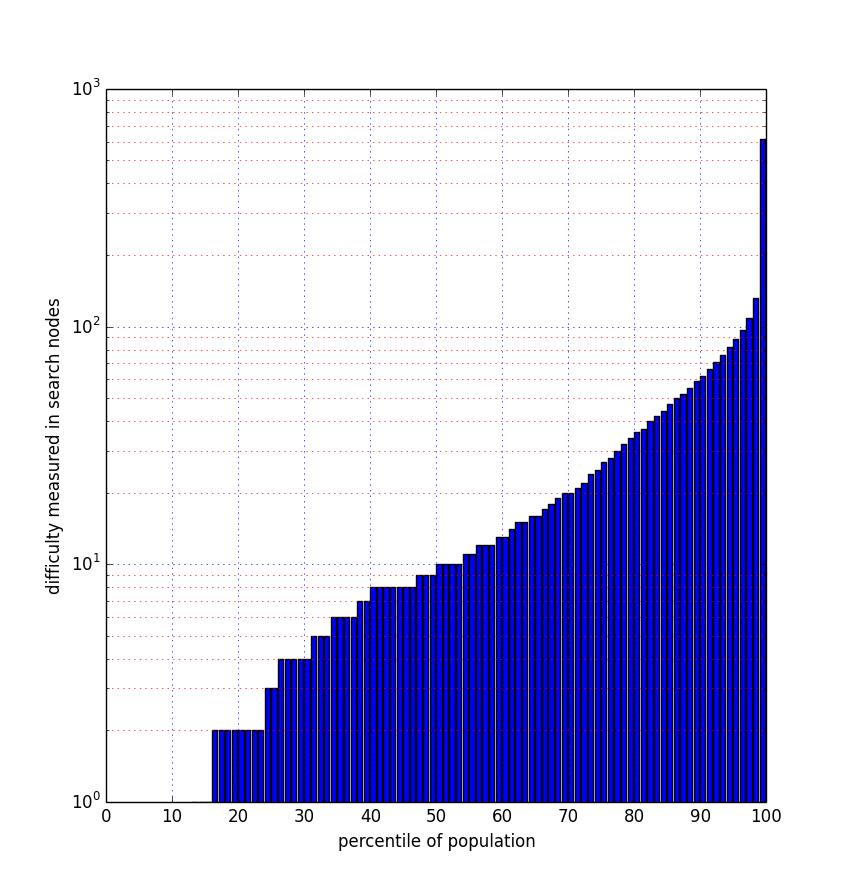
\includegraphics[height=11cm,width=9cm]{images/plots/aidsPercentileLog.png}
  \caption{SIP on Aids}
  \label{aidsNodes}
\end{minipage}%
\begin{minipage}[t]{.5\textwidth}
  \centering
  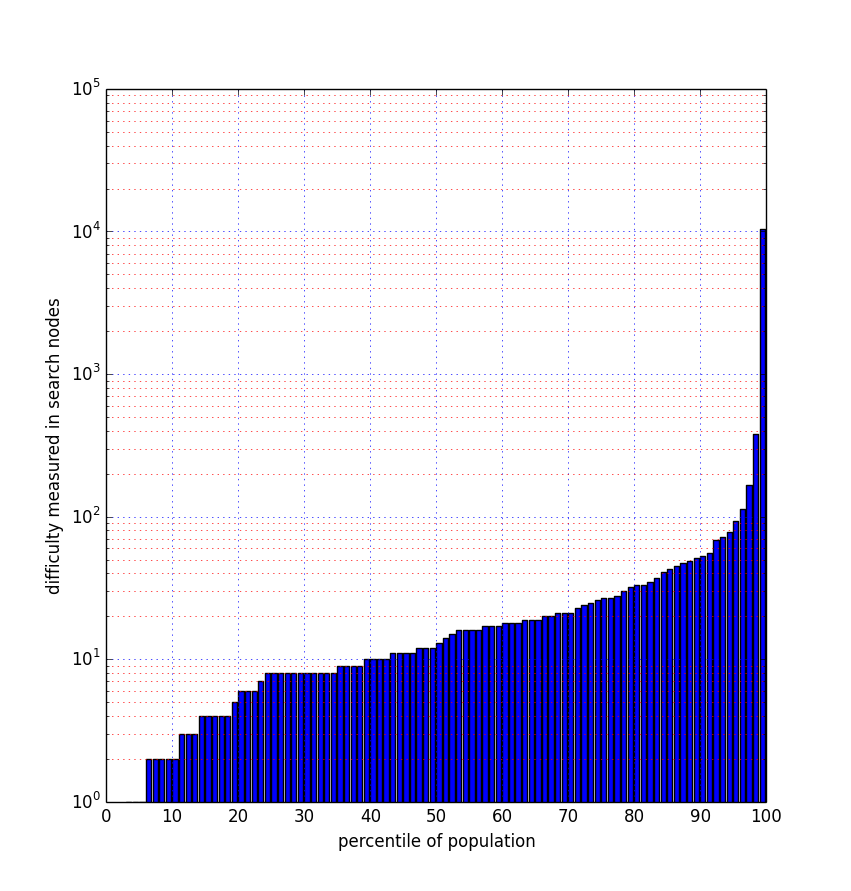
\includegraphics[height=11cm,width=9cm]{images/plots/pcmsPercentileLog.png}
  \caption{SIP on Pcms}
  \label{pcmsNodes}
\end{minipage}
\end{figure}
\begin{figure}
\centering
\begin{minipage}[t]{.5\textwidth}
  \centering
  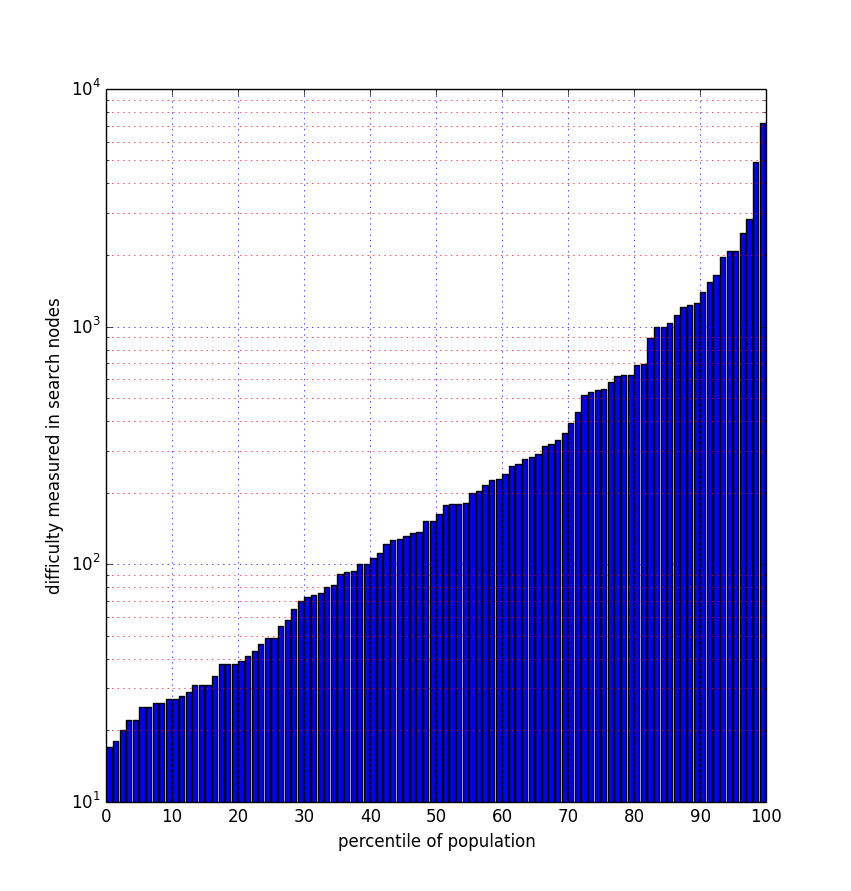
\includegraphics[height=11cm,width=9cm]{images/plots/pdbsPercentileLog.png}
  \caption{SIP on Pdbs}
  \label{pdbsNodes}
\end{minipage}%
\begin{minipage}[t]{.5\textwidth}
  \centering
  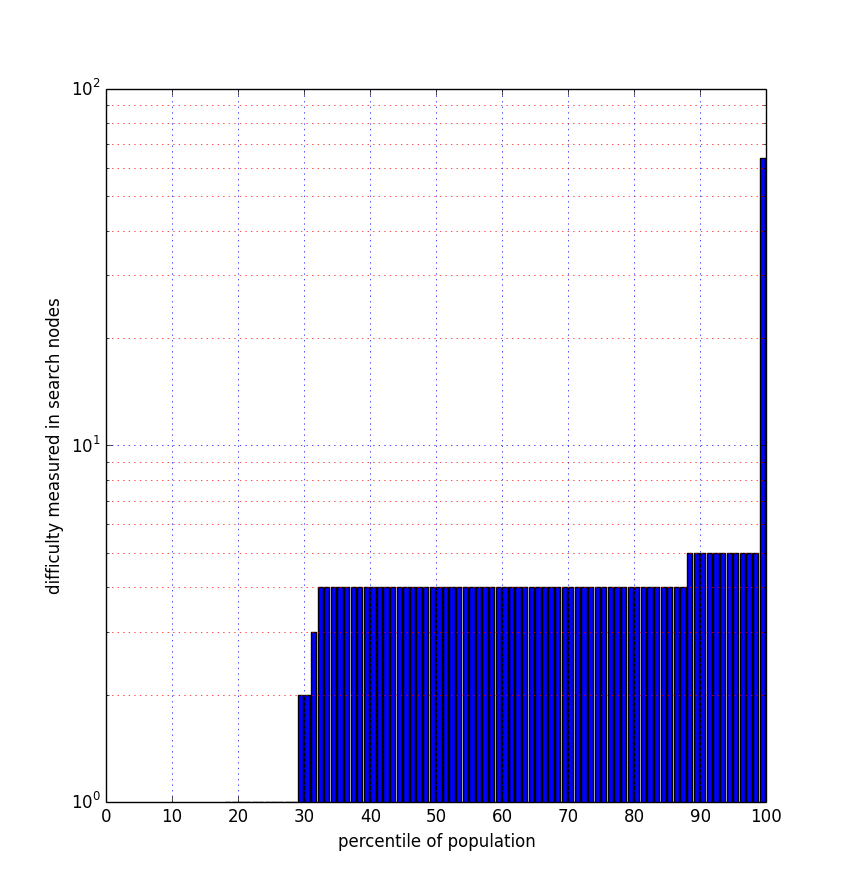
\includegraphics[height=11cm,width=9cm]{images/plots/ppigoPercentileLog.png}
  \caption{SIP on Ppigo}
  \label{ppigoNodes}
\end{minipage}
\end{figure}
%%%%

\subsection{Hardness of verification in terms of running time}
\label{subsec:hardnessVerifcTime}

Table \ref{table:cpuTime} shows the total time in milliseconds taken to solve all \gls{sip} instances of a given dataset. The time on the first row shows the total running time of Light Filters that includes file I/O, creating and instantiating objects and domains of variables, the filtering and the verification time. The second row shows the number of milliseconds taken to perform the filtering step and the third: the \gls{sip} algorithm. Note that the filtering step is performed for every sip instance, whereas verification is applied only on instances that were not rejected during filtering. The percentage of calls to sip for each dataset can be seen on Figure \ref{table:failures}.

The table shows that reading in the graphs from a file and instantiating the required objects and variables takes significantly more running time than filtering and verification for each dataset. 
This shows that further improving filtering and verification would not improve the performance of the algorithm much. Looking at the results from Pdbs, the dataset where verification was performed for every instance, we can see that even here verification is several times cheaper than file I/O and objects instantiation. We see that solving the subgraph isomorphism problem can not be described as ``too time consuming''.

For Ppigo and Pcms, filtering took more time than verification. Looking at the results for the Aids dataset, filtering and verification take almost the same time (filtering took 2,569 millis. and verification took 2,687 millis.). The 5,006 milliseconds spent on filtering for \gls{sip} problems in Pdbs was wasteful, because no instance was rejected (\ref{averageFailures}). Performing \gls{sip} algorithm on all 3,600 instances (\ref{table:dataSAT}) took 16,102 milliseconds, which makes 4.47 milliseconds per instance on average. During the analysis of the search effort, it was noticed that Pdbs is the hardest dataset. Achieving so fast verification time shows again that the four Big Data datasets are indeed very easy.

\begin{table}
\centering
\renewcommand{\arraystretch}{1.3}% Spread rows out...
\begin{tabular}{ |>{\centering\bfseries}m{1.2in} |>{\centering}m{0.5in}| >{\centering}m{0.5in}| >{\centering}m{0.5in}| >{\centering\arraybackslash}m{0.5in}|} 
\hline
 & \textbf{Aids} & \textbf{Pcms} & \textbf{Pdbs}  & \textbf{Ppigo} \\
\hline
total cpu T & 15,770 & 26,855 & 133,451 & 11,886 \\
\hline
total filtering T & 2,569 & 1,500 & 5,006 & 379 \\
\hline
total verification T & 2,687 & 1,013 & 16,102 & 51 \\
\hline
\end{tabular}
\caption{Total running time in milliseconds for each dataset}
\label{table:cpuTime}
\end{table}

Our investigation of the hardness of the four Big Data datasets, with respect to running time and number of search nodes, shows that all of them are easy and some of them (Ppigo) are particularly easy. The data obtained after the experiments shows that for Light Filters, the bottleneck of the performance of subgraph query processing is mainly I/O and objects initialization even for the dataset that involved executing verification for each instance (Pdbs). This suggests that the claim that solving the subgraph isomorphism problem for every instance takes substantial amount of time is not valid for the studied four datasets.

So far we discovered that although Aids, Pcms, Pdbs and Ppigo are commonly used by Big Data research for evaluation, they are of substandard quality. Each of the datasets claims that contains big number of complex graphs, but in practice all of them contain easy instances and two of the datasets contain large number of duplicates.
It was noted earlier that most of the subgraph query processing methods that implement the filtering-verification framework, were evaluated with some of these datasets. This puts into question their performance on datasets of standard quality and the superiority of current filtering-verification techniques over subgraph query processing techniques based only on verification.

As Light Filters method is evaluated only with the Big Data datasets, we can make conclusions on its performance only in comparison with the performance of other filtering-verification techniques. This is done in Section \ref{subsubsec:bigDataCompare}.


\section{Hardness of SAT vs UNSAT SIP instances}
The observation that the hardest instance of each dataset is UNSAT raises the following question: are \gls{unsat} \gls{sip} instances generally harder to solve than SAT SIP instances? The experiments described in this Section intend to investigate this.

The following eight plots below break each of the plots discussed in Section \ref{subsec:hardnessVerifcNodes} (namely \ref{aidsNodes}, \ref{pcmsNodes}, \ref{pdbsNodes} and \ref{ppigoNodes}) further down in terms of whether the SIP instances are \gls{sat} or \gls{unsat}. The blue plots represent all satisfiable SIP pairs for a dataset \emph{D}. Similarly, the red plots represent all unsatisfiable SIP instances of \emph{D}. For each \emph{D} (namely, for Aids, Pcms, Pdbs and Ppigo), the union of the blue plot (\gls{sat} \gls{sip}, left-hand side) and the red plot (\gls{unsat} \gls{sip}, right-hand side) gives the plot for the corresponding dataset discussed in Section \ref{subsec:hardnessVerifcNodes}.

Note that the plots on Figure \ref{fig:ppigoSatUnsat} contain only 4 bars each, i.e. the data is divided into quartiles instead of percentile. Here, each bar represents 25\% of all instances of a category (\gls{sat}/\gls{unsat}). For example, the left plot shows that the lowest quartile of the \gls{sat} \gls{sip} calls takes no more than 4 nodes to solve, as it is also true for the second quartile. We changed the percentile representation for this dataset, because the number of \gls{sat} and \gls{unsat} \gls{sip} (61 and 39 respectively, Table \ref{table:dataSAT}) instances is too small to be scaled to percentiles.
%%% SAT vs UNSAT in terms of search nodes
\begin{figure}
\centering
\begin{minipage}[t]{.5\textwidth}
  \centering
  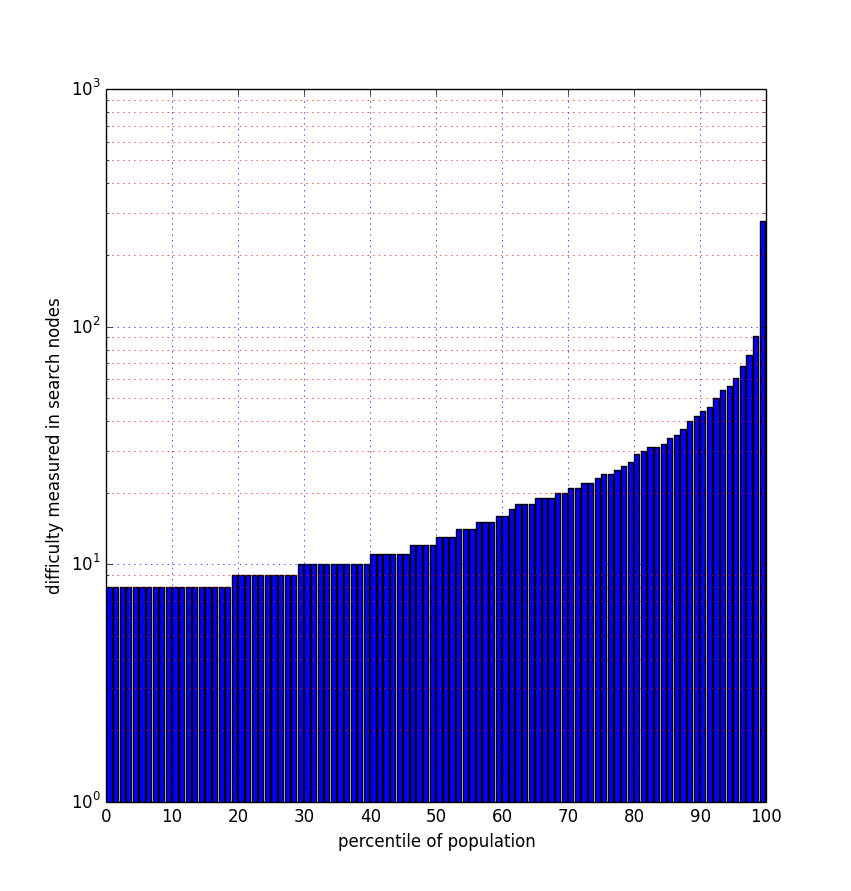
\includegraphics[height=11cm,width=9cm]{images/plots/aidsSAT.png}
\end{minipage}%
\begin{minipage}[t]{.5\textwidth}
  \centering
  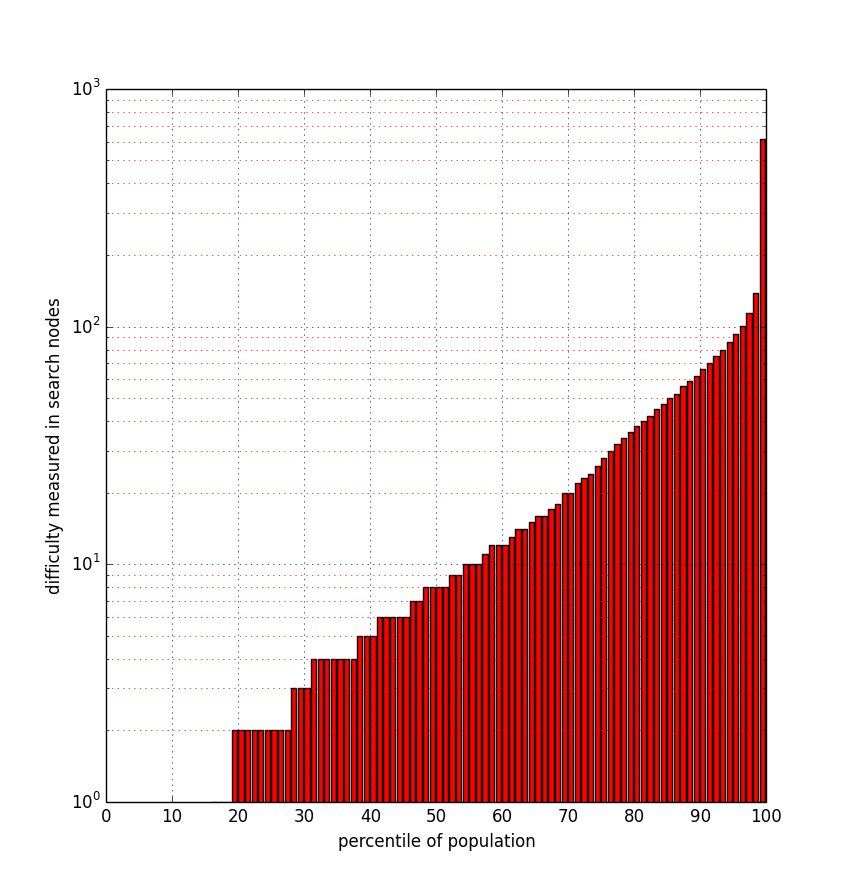
\includegraphics[height=11cm,width=9cm]{images/plots/aidsUNSAT.png}
\end{minipage}
\caption{Search effort for \gls{sat}(blue, left) \gls{unsat}(red, right) \gls{sip} instances in Aids}
\label{fig:aidsSatUnsat}
\end{figure}
\begin{figure}
\centering
\begin{minipage}[t]{.5\textwidth}
  \centering
  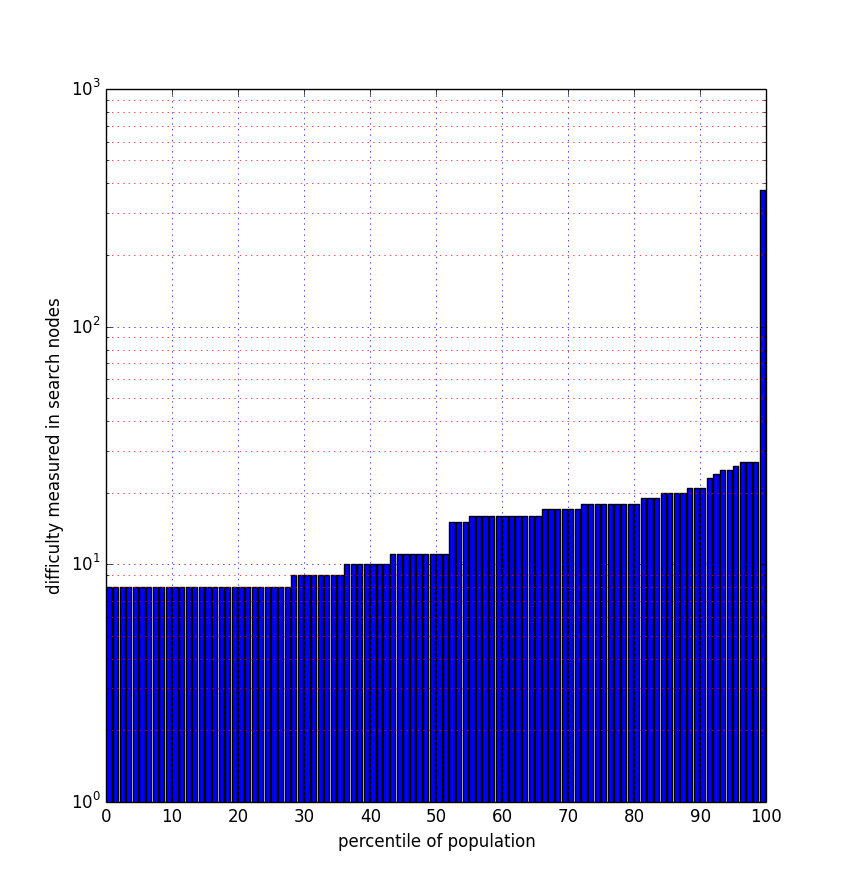
\includegraphics[height=11cm,width=9cm]{images/plots/pcmsSAT.png}
\end{minipage}%
\begin{minipage}[t]{.5\textwidth}
  \centering
  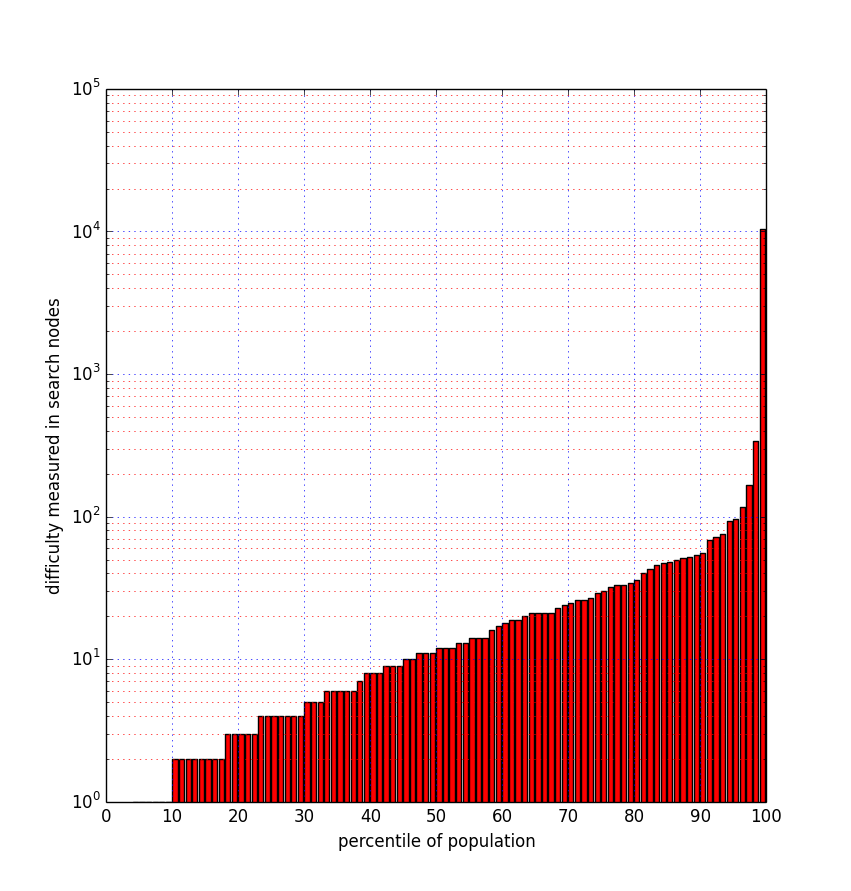
\includegraphics[height=11cm,width=9cm]{images/plots/pcmsUNSAT.png}
\end{minipage}
\caption{Search effort for \gls{sat}(blue, left) \gls{unsat}(red, right) \gls{sip} instances in Pcms}
\label{fig:pcmsSatUnsat}
\end{figure}
\begin{figure}
\centering
\begin{minipage}[t]{.5\textwidth}
  \centering
  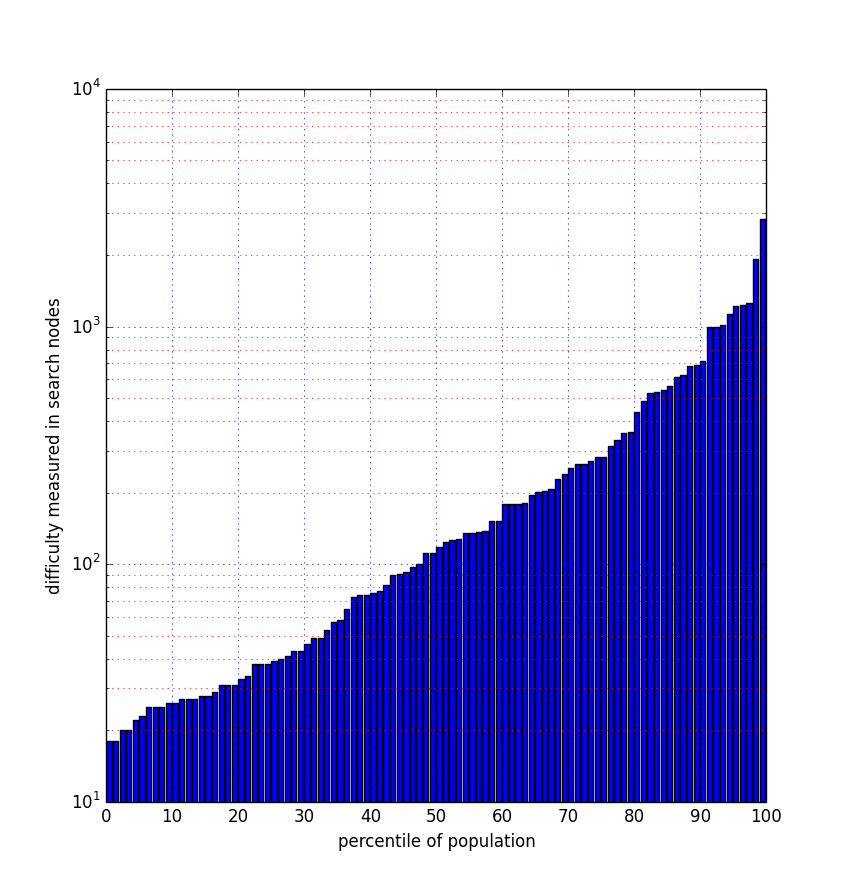
\includegraphics[height=11cm,width=9cm]{images/plots/pdbsSAT.png}
\end{minipage}%
\begin{minipage}[t]{.5\textwidth}
  \centering
  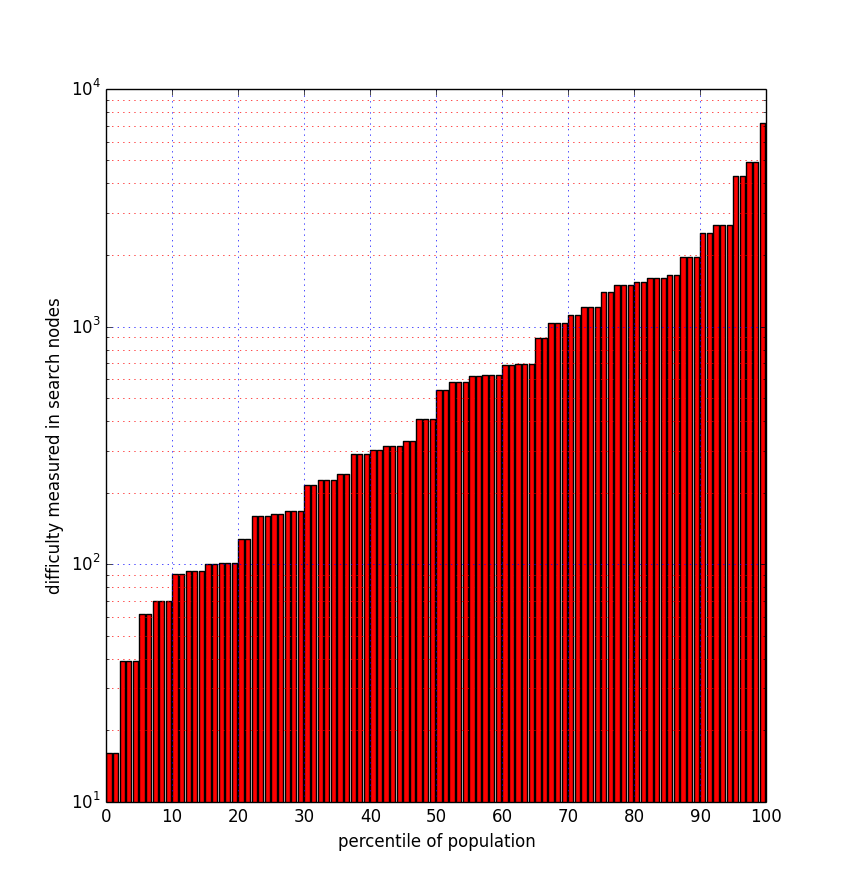
\includegraphics[height=11cm,width=9cm]{images/plots/pdbsUNSAT.png}
\end{minipage}
\caption{Search effort for \gls{sat}(blue, left) \gls{unsat}(red, right) \gls{sip} instances in Pdbs}
\label{fig:pdbsSatUnsat}
\end{figure}
\begin{figure}
\centering
\begin{minipage}[t]{.5\textwidth}
  \centering
  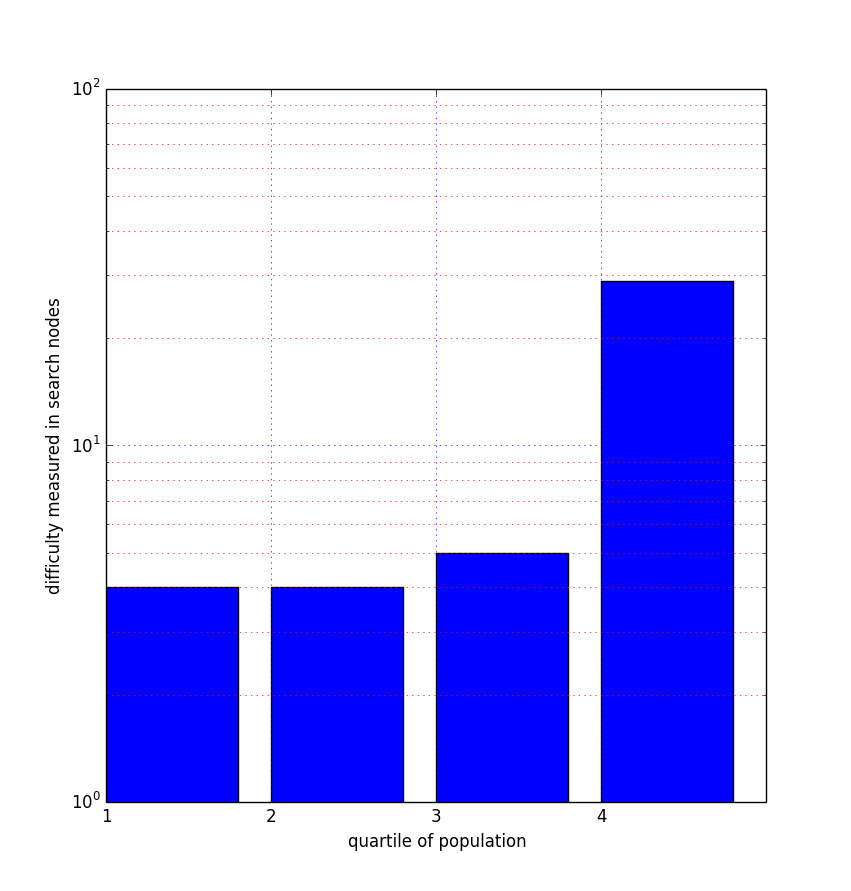
\includegraphics[height=11cm,width=9cm]{images/plots/ppigoSAT.png}
\end{minipage}%
\begin{minipage}[t]{.5\textwidth}
  \centering
  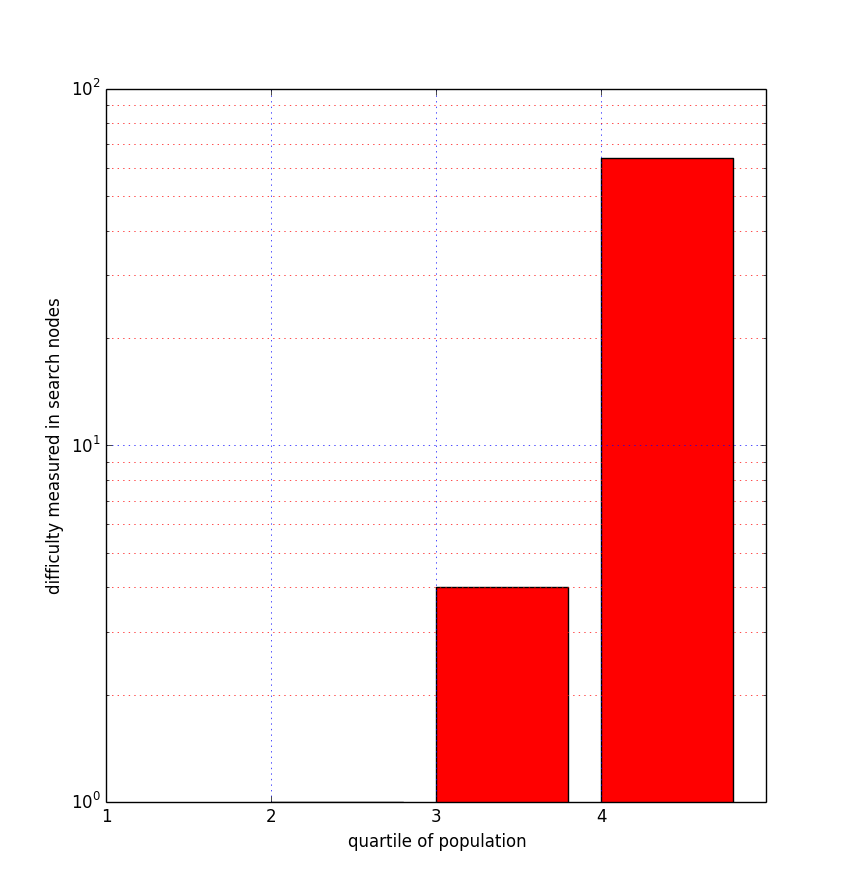
\includegraphics[height=11cm,width=9cm]{images/plots/ppigoUNSAT.png}
\end{minipage}
\caption{Search effort for \gls{sat}(blue, left) \gls{unsat}(red, right) \gls{sip} instances in Ppigo}
\label{fig:ppigoSatUnsat}
\end{figure}
%%%%

Table \ref{table:SATUNSATnodes} presents statistics in terms of number of search nodes for \gls{sat} (blue columns) and \gls{unsat} (red columns) instances. For instance, the Table shows that for Aids, the total number of search nodes taken to solve all \gls{sat} \gls{sip} instances is 437,108, and the total number of search nodes taken to solve all \gls{unsat} \gls{sip} instances is 2,295,724. Using these Figures, we derive that the total number of search nodes taken to solve all \gls{sip} instances in Aids is the sum of those two numbers, which is equal to 2,732,832. Table \ref{table:dataSAT} also shows the number of instances and percent from each category(SAT/UNSAT). The Table tells us that the reason for the large difference in terms of search effort between SAT and UNSAT instances is that 91\% of all instances are UNSAT (almost ten times more than SAT). The two tables and the 8 figures show that:

\begin{itemize}
\item In Aids, Pcms and Ppigo, the easiest percentile of \gls{unsat} \gls{sip} instances requires less number of search nodes than the easiest percentile of \gls{sat} \gls{sip} instances. The hardest percentile of \gls{unsat} \gls{sip} takes bigger number of search nodes than the hardest percentile of \gls{sat} \gls{sip} instances.

\item In Pdbs, there is a big difference in terms of search effort between SAT and UNSAT problems. For example, \gls{sat} instances are easier for every percentile of the targets (\ref{fig:pdbsSatUnsat}). The tabulated results on Figure \ref{table:SATUNSATnodes} confirm this observation. On average, SAT instances are 3 times easier than UNSAT, the SAT instances median is more than 4 times smaller than the UNSAT instances median and the number of search nodes taken to solve the hardest SAT instance (2,845) is much less than the number of search nodes taken to solve the hardest UNSAT instance (7,152).

\item Table \ref{table:SATUNSATnodes} shows that in Pdbs, the total search effort taken to solve UNSAT problems is bigger (894,260 search nodes taken in total for SAT and 854,720 search nodes in total taken for UNSAT problems). However, Table \ref{table:dataSAT} shows that \gls{sat} \gls{sip} consists of 77.22\% of all instances in Pdbs. Therefore, the large search effort of SAT SIP problems for pdbs is due to their substantially larger number compared to UNSAT problems and in practice, \gls{unsat} \gls{sip} was much more difficult to solve than \gls{sat} \gls{sip} for this dataset. This is confirmed by the average search nodes figures (the second row in Table \ref{table:SATUNSATnodes}), where a SAT instance is on average 3 times easier to solve than an UNSAT instance.

\item Pcms is composed of mostly \gls{unsat} \gls{sip} instances (\ref{table:dataSAT}, \ref{averageFailures}). Similarly to Aids, this is the reason why the total number of search nodes for all \gls{unsat} problems is considerably larger than the number of search nodes for all \gls{sat} problems (\ref{table:SATUNSATnodes}). However, the hardest \gls{sat} problem is substantially easier than the hardest \gls{unsat}. The difference is 10,092 search nodes, where the SAT problem takes 378 search nodes to be solved (\ref{table:SATUNSATnodes}) and it is \gls{sip} (``\#32\_1CY1.cm.A.out'', ``\#1CY0.cm.A.cmap''), solved for 4 milliseconds. Average search nodes figures also show that a SAT instance is on average 5 times easier to solve than an UNSAT instance(the second row in Table \ref{table:SATUNSATnodes}).

\item 61\% of all instances in Ppigo are \gls{sat} (\ref{table:dataSAT}, \ref{averageFailures}) and this is the main reason why the total SAT SIP search effort is larger than the UNSAT SIP search effort. The average search effort displayed in Table \ref{table:SATUNSATnodes} shows that SAT and UNSAT SIP instances are similarly hard on average for this dataset.
\end{itemize}


\newcolumntype{g}{>{\columncolor{red!15}}r}
\newcolumntype{b}{>{\columncolor{blue!15}}r}
\begin{table}
\centering
        \renewcommand{\arraystretch}{1.5}% Spread rows out...
        \begin{tabular}{c|bg|bg|bg|bg|bg|}
            \cline{2-11}
            &
             \multicolumn{2}{c}{\textbf{Total}} & 
             \multicolumn{2}{|c}{\textbf{Average}} & 
             \multicolumn{2}{|c|}{\textbf{Median}} & 
             \multicolumn{2}{c}{\textbf{Minimum}} & 
             \multicolumn{2}{|c|}{\textbf{Maximum}} \\
              \hline
            \cline{2-11}
             \hline
            % & SAT & UNSAT & SAT & UNSAT & SAT & UNSAT & SAT & UNSAT & SAT & UNSAT\\
            \multicolumn{1}{|c|}{\textbf{Aids}}  &437,108  &2,295,724 &21 &10.4   &13  &0   &9  &0  &279   &619 \\
            \multicolumn{1}{|c|}{\textbf{Pcms}}  &13,644   &133,276   &23 &110.3  &17  &9   &9  &0  &378   &10,470 \\
            \multicolumn{1}{|c|}{\textbf{Pdbs}}  &894,260  &854,720   &322 &1,042.3 &123 &544 &18 &17 &2,845 &7,152 \\
            \multicolumn{1}{|c|}{\textbf{Ppigo}} &714      &312       &6.932  &5.8    &6   &2   &5  &0  &30    &65 \\
            \hline
        \end{tabular}
        \caption{Number of nodes of search effort for each dataset. Blue for solvable and red for unsolvable SIP instances}
        \label{table:SATUNSATnodes}
    \end{table}

\section{Comparison with Big Data algorithms}
\label{subsubsec:bigDataCompare}
We make a comparison of Light Filters with a selection of ``well-established'' subgraph query processing algorithms, namely CT-Index \cite{ctindex}, gCode \cite{gcode}, Grapes \cite{GRAPES}, tree+$\Delta$ \cite{tree+delta>=graph}, GGSX \cite{graphgrepsx} and gIndex \cite{freqStructBasedIndexing1}. Their evaluation is described in \cite{foteini}. All of these algorithms implement the filtering-verification framework with heavy filtering approach, using an index structure, and run \gls{sip} algorithm during verification, that is VF2 \cite{vf2} or a modification of it. The work in \cite{foteini} uses the same datasets and the same machine as us for its experiments. The comparison is made first with respect to running time and then with respect to filtering strength.

For Aids, the fastest of the evaluated algorithms is Grapes \cite{GRAPES}. Filtering took 8 seconds and verification- about 600 milliseconds. It took us 2,569 milliseconds for filtering (\ref{table:cpuTime}), but verification was four times slower (2,687 milliseconds). Light Filters approach has slower verification than CT-Index, but much faster filtering. The algorithms with slowest filtering and verification time, evaluated in \cite{foteini}, are gIndex and tree+$\Delta$ (15000 and 1500 seconds for filtering, 8 and 40 seconds for verification respectively \cite{foteini}). Light Filters is several times better than them on each stage. 

In the study described in \cite{foteini}, it was observed that for Pcms and Ppigo, for four of the evaluated algorithms filtering never finished executing. Interestingly, Pcms and Ppigo are the only two datasets that are composed by mainly SAT instances (Figure \ref{averageFailures}). Table \ref{table:cpuTime} shows that the performance of the Light Filters is incomparably faster, where filtering of all instances took only 1,500 milliseconds for Pcms and 5,006 milliseconds for Pdbs. The results in \cite{foteini} show that the only two algorithms, that can solve these datasets, are Grapes and GGSX \cite{graphgrepsx}. The running time of both of them for both filtering and verification is slower than the running time of Light Filters. We can deduce that for solving Pcms and Ppigo, Light Filters is the single best technique.

We get similar results as for the Aids dataset, when we compare running time of Light Filters and the other six techniques for Pdbs.

Below we give a summary of the main discoveries while investigating performance running time.
\begin{itemize}
\item With respect to running time, for the two of the datasets, that have mainly SAT instances, Light Filters is the single best technique. In terms of running time of filtering, Light Filters is the fastest. This is not surprising. This result is not surprising. The filtering part of our method constitutes of five simple tests (Section \ref{sec:trivialFails}), whereas the filtering of each of the other methods follows the classical principles of the filtering-verification paradigm. In terms of verification time, Light Filters is neither the fastest, nor one of the slowest. The algorithms evaluated in \cite{foteini} have an additional overhead that is not present in our approach, which is the size of the index that has to be stored. However, the cost of the filtering procedures of Light Filters is paid every time no matter of the dataset, whereas the index built during filtering of classical filtering-verification methods can be built upfront and reused as long as the database does not change.
\item It was previously shown that the maximum bound on effectiveness of filtering is defined by the number of UNSAT SIP instances in the dataset. Four of the indexing algorithms, evaluated in \cite{foteini}, never finish execution for Pcms and Ppigo, which are mainly composed of SAT SIP instances. Therefore, executing expensive filtering algorithms for such datasets is difficult to justify both in terms of effectiveness and efficiency.
\end{itemize}

%Let us look at the results obtained after we ran experiments on CT-Index with the Aids dataset. Our results for CT-Index are shown in Table \ref{table:runningTime} and the running time of Light Filters when run with Aids is shown in the first column of Table \ref{table:cpuTime}. Let us compare Light Filters with the best verification running time observed for CT-Index, that is the one in row 15, where verification took 5.9 seconds. To take the reusability property of database indices into an account, we compare the sum of the filtering and verification running time of Light Filters only with the verification time of CT-Index. Our approach still beats the best CT-Index with almost a second.

We now compare the filtering performance of Light Filters with the six techniques.

To make the filtering performance of Light Filters comparable with the results in the work described in \cite{foteini}, we used formula \ref{eq:fpratio}, discussed in Section \ref{subsec:ctindexEval} to calculate the FP ratio of Light Filters for every of the four datasets. Table \ref{table:FPratioLightFilters} shows our results.

First, we can deduce that formula \ref{eq:fpratio} behaves as we discussed in Section \ref{subsec:ctindexEval}. For datasets where filtering removed 0 or close to 0 instances, like Pdbs and Ppigo, the value of FP ratio depends only on the number of SAT instances in the dataset and it does not show that the filtering performed poorly. Figure \ref{averageFailures} shows that filtering removed 0 instances from the Pdbs dataset, however, the FP ratio for Pdbs shows great filtering performance of 0.23 (Table \ref{table:FPratioLightFilters}). Filtering was most successful for Aids (Figure \ref{averageFailures}), but according to Table \ref{table:FPratioLightFilters}, it is worst for Aids. This data further supports our observations in Section \ref{subsec:ctindexEval} that formula \ref{eq:fpratio}, used to evaluate the filtering power of some filtering-verification algorithms \cite{foteini}, can be used only in order to compare performance of different filtering methods, executed on the same datasets, and the FP ratio values on their own do not suggest anything accurate about the effectiveness of a given filtering algorithm. 

According to the results, published in \cite{foteini}, the five simple failure tests do not perform worse than the studied filtering-verification techniques in that publication (which are considered to be ``well established indexing methods'' \cite{foteini}). For instance, the best FP ratio for Aids was obtained by tree+$\Delta$ with value 0.2 \cite{foteini} and the worst FP ratio is achieved by 3 algorithms (Grapes, CT-index, gCode) with value 0.8 \cite{foteini}. The FP ratio of Light Filters for Aids is 0.73 (Table \ref{table:FPratioLightFilters}). The best FP ratio for Pdbs in \cite{foteini} is obtained by Grapes and has the value 0.04 \cite{foteini}, the worst value is 0.3 \cite{foteini}, which is slightly worse than the FP ratio obtained by Light Filters of value 0.23 (Table \ref{table:FPratioLightFilters}). For Pcms and Ppigo, we can compare only two algorithms with Light Filters, because only they finished execution. Here, Light Filters is significantly better than the worst of the algorithms (Table \ref{table:FPratioLightFilters}), that has FP ratio equal to 0.7 \cite{foteini}, but worse compared to the best algorithm that has FP ratio equal to 0.2 \cite{foteini}. The results are similar when comparing results from the Ppigo results of \cite{foteini} and the figures in Table \ref{table:FPratioLightFilters}.

\begin{itemize}
\item The comparison of the filtering methods implemented in Light Filters with six well-established filtering-verification methods \cite{foteini} using the same four datasets, shows that small, easy to compute filtering mechanisms (Light Filters) can in some cases give better filtering performance than subgraph query processing methods that employ heavy index structures. %If one looks at the running time of filtering, Light Filters beats each of the other algorithms by several orders of magnitude.
\end{itemize}

\begin{table}
\centering
\renewcommand{\arraystretch}{1.3}% Spread rows out...
\begin{tabular}{ |>{\centering\bfseries}m{0.7in} |>{\centering\arraybackslash}m{0.7in}|} 
\hline
& \textbf{FP Ratio} \\
\hline
\textbf{Aids} & 0.73 \\
\hline
\textbf{Pcms} & 0.44 \\
\hline
\textbf{Pdbs} & 0.23 \\
\hline
\textbf{Ppigo} & 0.36 \\
\hline
\end{tabular}
\caption{FP ratio of filtering of Light Filters for each of the datasets}
\label{table:FPratioLightFilters}
\end{table}

%It was discovered that the Big Data datasets are of poor quality. Two of the datasets have targets that are copied multiple times each. All four datasets contain very easy \gls{sip} instances. The hardest of the datasets is pdbs. Even with the hardest dataset, a \gls{sip} instance took only 4.47 milliseconds to be solved on average. Verification for 50\% of the instances in pdbs took much less than 90 \glspl{sn}, the most expensive \gls{sip} problem costs 10,470 \glspl{sn}. Surprising finding was that the datasets can be easily kept in memory. Big Data is much smaller than what we initially expected. Beneficial future work in this area would be to develop better quality, much bigger and harder datasets. 
   
\chapter{Conclusion and Future work}
This Chapter presents a summary of this work. It starts by outlining the major steps carried out and what each of them suggests. The second part of the Chapter, discusses opportunities for future work, which could follow on from the project. 

\section{Project Summary}
We investigated the subgraph query processing problem and we first looked at two currently existing methods to solve it. The filtering-verification paradigm, is a new approach, considered as very effective among the area of Big Data research. The second subgraph query processing technique is to solve the subgraph isomorphism problem for every instance.

We analysed a well-established filtering-verification technique, called CT-Index \cite{ctindex} and CP15 \cite{CP2015}- a new subgraph isomorphism problem algorithm that is shown to be the fastest when compared with other well-established algorithms. After the review of the literature, we observed that all filtering-verification-based techniques are mainly focused in developing new filtering methods, while reusing the same subgraph isomorphism algorithm for verification, which was proved to be of substandard performance.

The next step was to investigate the area of developing filtering methods by designing and implementing such techniques. We implemented a filtering framework with two methods for filtering and candidates extraction, namely Path Index and Path-Subtree Index. Path Index follows a common feature construction algorithm and Path-Subtree Index is a new technique, introduced by us. Our theoretical analysis showed that Path-Subtree Index prunes at least as many instances as Path Index, but it has higher complexity and storage requirements than Path Index. Both techniques were shown to be effective, but too slow to be used in practice and we suggested possible ways to lower their complexity.

We introduced Light Filters- a new subgraph query processing technique that implements a modification of the filtering-verification paradigm. Light Filters does not employ any index structure. Filtering is consists of five simple failure tests and verification is performed by a subgraph isomorphism algorithm, based on the simplest of the Glasgow algorithms \cite{CP2015}. We ran experiments with Light Filters on four commonly used Big Data datasets. The results from the experiments show that the datasets are of substandard quality. Moreover, they contain so easy instances, that it is difficult to make major conclusions on the effectiveness of Light Filters for subgraph query processing and puts into question the performance of all filtering-verification based algorithms that are evaluated only with these datasets.

We discovered that the four Big Data datasets can be easily kept in memory of a standard laptop without the usage of additional hardware. This shows that Aids, Pcms, Pdbs and Ppigo are not adequate representatives of Big Data datasets, nonetheless they are treated as such. It raises the question of how Big Data filtering-verification algorithms, would behave when evaluated with bigger and more complex datasets.

We ran experiments on Light Filters using the same datasets and setup that were used in \cite{foteini}. This allowed us to compare Light Filters with a selection of the best existing filtering-verification techniques. With respect to filtering performance, the results showed that some of these techniques were outperformed by Light Filters. In terms of filtering running time, Light Filters is the fastest. In terms of verification running time, Light Filters is the technique with the fastest running time. 

In terms of effectiveness of filtering, although Light Filters uses very simple tests, it manages to beat some of the indexing techniques it was compared with for each of the datasets. This shows that light filtering approaches have a potential to be as good as heavy filtering techniques in terms of pruning UNSAT instances, but also much faster in terms of running time.

We observed that for datasets that are composed of mainly SAT SIP instances, indexing methods are not only highly inefficient (typically never finish execution), but also bound to be of less effectiveness. For such datasets, it is better to use approaches like Light Filters, that emphasize on verification and use fast and simple filtering techniques.

%Filtering is bound to work only in the area of UNSAT SIP instances. Consequently, when most of the instances of the dataset are SAT, filters can be more an overhead than help. The SIP algorithm, performed during verification, can both identify SAT and UNSAT problems. Therefore, constructing sophisticated filtering would give little gain, if any, but implementing fast and smart \gls{sip} would improve the performance significantly.  

We did experiments to find out whether \gls{sat} problems are generally easier than \gls{unsat} problems that were not rejected by filtering. We got varied answers for each dataset, therefore no definite conclusion about this can be made. What was observed is that for each of the datasets, the hardest and the easiest instances in terms of \glspl{sn} are both \gls{unsat}.  

\section{Future Work}
This work put into question the performance of subgraph query processing methods based on the filtering-verification paradigm, mainly because of the substandard quality of the datasets, used as benchmarks. This leads to the following possible extension of this work. %Filtering-verification based algorithms could be tested with datasets that are good representatives of the real demand of Big Data in terms of size and complexity.
One could develop new datasets that consist of harder subgraph isomorphism problem instances. There is currently existing work that shows how to generate ``really hard'' random instances for subgraph isomorphism problem \cite{patrick:2015}. A future project could focus on creating large datasets with this methodology and then conduct experimental evaluation of filtering-verification based algorithms (including Light Filters) with these datasets. This could give better understanding of the performance of subgraph query processing methods with datasets that are possibly better representatives of the real demand of Big Data in terms of size and complexity.

Light Filters technique was shown to be as good as, or outperform classical filtering-verification techniques in several aspects. Future extension of this work could investigate what makes the current filtering tests so effective and how to extend the filtering by adding more tests.

It was shown that the effectiveness of subgraph query processing algorithms depends on the nature of the datasets \cite{CP2015}. Future extension of this work could focus on creating a large framework that predicts the difficulty of an instance before solving it and depending on its difficulty, chooses an appropriate filtering and verification methods. There is an existing work that gives a formula how to calculate hard instances, given in \cite{Gent:1996}, and an existing work that investigates where the hard problems are \cite{Cheeseman:1991}.

%%%%%%%%%%%%%%%%%%%%
%   BIBLIOGRAPHY   %
%%%%%%%%%%%%%%%%%%%%

\bibliographystyle{plain}
\bibliography{bib}
\printglossary
\printglossary[type=\acronymtype]
\end{document}
